\documentclass{ieeeaccess}
\usepackage{cite}
\usepackage{amsmath,amssymb,amsfonts}
\usepackage{url}
\usepackage{multirow}
\usepackage{float}
\usepackage{graphicx}
\usepackage{textcomp}
\usepackage{adjustbox}
\usepackage[normalem]{ulem}
\useunder{\uline}{\ul}{}
\usepackage{rotating}
\usepackage{longtable}
\usepackage{booktabs}
\usepackage{array}
\usepackage{algorithm}
\usepackage{algpseudocode}
\usepackage{hyperref}

\def\BibTeX{{\rm B\kern-.05em{\sc i\kern-.025em b}\kern-.08em
    T\kern-.1667em\lower.7ex\hbox{E}\kern-.125emX}}
\begin{document}
\history{Date of publication xxxx 00, 0000, date of current version xxxx 00, 0000.}
\doi{10.1109/ACCESS.2023.0322000}

\title{HetGNN-KGAT: Enhancing Personalized Course Recommendation in MOOCs with Knowledge Graph Attention Networks}

% author
\author{
\uppercase{Thu Nguyen}\authorrefmark{1,3,*},
\uppercase{Dat Do}\authorrefmark{1,3,*},
\uppercase{Huong Vi}\authorrefmark{1,3,*},
\uppercase{Khoa Tan VO}\authorrefmark{1,3},
\uppercase{Thu-Thuy Ta}\authorrefmark{1,3},
\uppercase{Mong-Thy Nguyen Thi}\authorrefmark{1,3},
\uppercase{Phuc Nguyen}\authorrefmark{2.3},
\uppercase{Hong-Tri Nguyen}\authorrefmark{4},
\uppercase{Tu-Anh Nguyen-Hoang}\authorrefmark{1,3}
}

\address[1]{Faculty of Information Science and Engineering, University of Information Technology, Ho Chi Minh City, Vietnam}
\address[2]{Faculty of Information Systems, University of Economics and Law, Ho Chi Minh City, Vietnam}
\address[3]{Vietnam National University, Ho Chi Minh City, Vietnam}
\address[4]{Aalto University, Finland}
\address[*]{These authors contributed equally}
\tfootnote{This research was supported by The VNUHCM-University of Information Technology's Scientific Research Support Fund.}

\markboth
{Thu Nguyen  \headeretal: HetGNN-KGAT: Knowledge Graph-Aware Course Recommendation in MOOCs}
{Thu Nguyen  \headeretal: HetGNN-KGAT: Knowledge Graph-Aware Course Recommendation in MOOCs}

\corresp{Corresponding author: Thu Nguyen (e-mail: thunta@uit.edu.vn, n240204@grad.uit.edu.vn) and Hong-Tri Nguyen (e-mail: hong-tri.nguyen@aalto.fi).}

\begin{abstract}
The rise of Massive Open Online Courses (MOOCs) has expanded educational access, but personalized course recommendation is challenged by sparse interaction data and complex learner-item relationships. This paper proposes HetGNN-KGAT, a framework integrating Heterogeneous Graph Neural Networks (HetGNN) for link prediction in a heterogeneous information network (HIN) and Knowledge Graph Attention Networks (KGAT) for recommendation enhancement. HetGNN outperforms traditional methods Listwise Deletion, Statistical Imputation, and ML-based Imputation by achieving complete and consistent data quality, while KGAT leverages relational structures. Evaluated on the MOOCCubeX dataset, HetGNN-KGAT shows improvements of up to 23.55\% in MAP, 11.37\% in F1-score, and 27.70\% in NDCG compared to baselines CBF, DeepFM, BPRMF, UPGPR, and KGAT in simulated scenarios. In real-world scenarios, enhancements reach up to 7.82\% in MAP, 3.73\% in F1-score, and 9.24\% in NDCG. The approach suggests a practical benefit in managing data sparsity and offers insights for advancing adaptive educational technologies.
\end{abstract}

\begin{keywords}
Educational technology, Heterogeneous graphs, Knowledge graphs, MOOC recommendation, Personalized learning.
\end{keywords}

\titlepgskip=-21pt

\maketitle

\section{Introduction}
\label{sec:introduction}
MOOCs have gained prominence in education over the past decade, providing millions of learners worldwide with access to diverse knowledge irrespective of spatial or temporal constraints. Platforms such as XuetangX, Coursera, and edX offer courses spanning foundational sciences to specialized skills, catering to a wide range of learners \cite{qaffas2020towards}. This accessibility supports lifelong learning and skill development in the digital era, marking a notable presence in modern education. However, the growth of MOOCs presents challenges, including sparse interaction data and low completion rates, typically ranging from 5-15\% \cite{jordan2014initial_trend_mooc}. These issues complicate course selection, reducing learner engagement and highlighting the need for effective recommendation systems.

% Discussing challenges in personalized recommendation
Personalized course recommendation in MOOCs is limited by data sparsity, cold-start problems, and the complex relationships among learners, courses, videos, and forums. Traditional methods like Collaborative Filtering (CF) and Content-Based Filtering (CBF) face difficulties with incomplete data and fail to fully capture relational structures \cite{mustafeez2024comprehensive}. Recent studies indicate that graph-based approaches, such as those using knowledge graphs, may address some of these limitations \cite{wang2019kgat}. However, these approaches often struggle with dynamic optimization and the integration of heterogeneous data, necessitating advanced methods to model complex interactions and improve recommendation accuracy.

% Bridging to data imputation methods
To tackle the challenge of data sparsity, a critical barrier to effective recommendation systems, various imputation methods have been explored in the context of MOOCs. Techniques such as Listwise Deletion, Statistical Imputation, and Machine Learning-based Imputation (e.g., KNN) have been employed to address missing data. Listwise Deletion \cite{Rubin2019statistical_analysis_missing_data} discards incomplete records, which may lead to substantial data loss. Statistical Imputation \cite{van2011mice}, such as mean or mode substitution, relies on simplistic assumptions and can introduce bias. Machine Learning-based methods, like KNN \cite{troyanskaya2001missingDNA}, utilize data patterns but may struggle with complex, nonlinear relationships in heterogeneous MOOC data. These limitations underscore the need for a robust framework that not only addresses data sparsity but also leverages the relational structures inherent in MOOC ecosystems to enhance recommendation performance.

% Introducing the proposed framework
The proposed HetGNN-KGAT framework provides a structured approach to enhancing recommendation systems in MOOC platforms by integrating HetGNN and KGAT. This methodology leverages the relational structures and node content of HetGNN to address data sparsity through effective link prediction and data imputation, while KGAT captures complex learner-course interactions to improve recommendation accuracy. The workflow of the framework, illustrated in the overview of the HetGNN-KGAT method (Figure \ref{fig:overview_hetgnn_kgat_method}), consists of four main stages: Data collection, Preprocessing (with a focus on HetGNN-based imputation), Recommendation model (utilizing the KGAT algorithm as the central technique), and Performance analysis. Based on graph-based learning principles, this process employs HetGNN to handle data imputation and KGAT to generate personalized recommendations, overcoming the limitations of traditional imputation and recommendation methods. A detailed examination of these components, including their theoretical foundations, implementation procedures, and practical steps, is provided in the subsequent theoretical background section to facilitate understanding and application of the proposed framework.

\begin{figure*}[h]
\centering
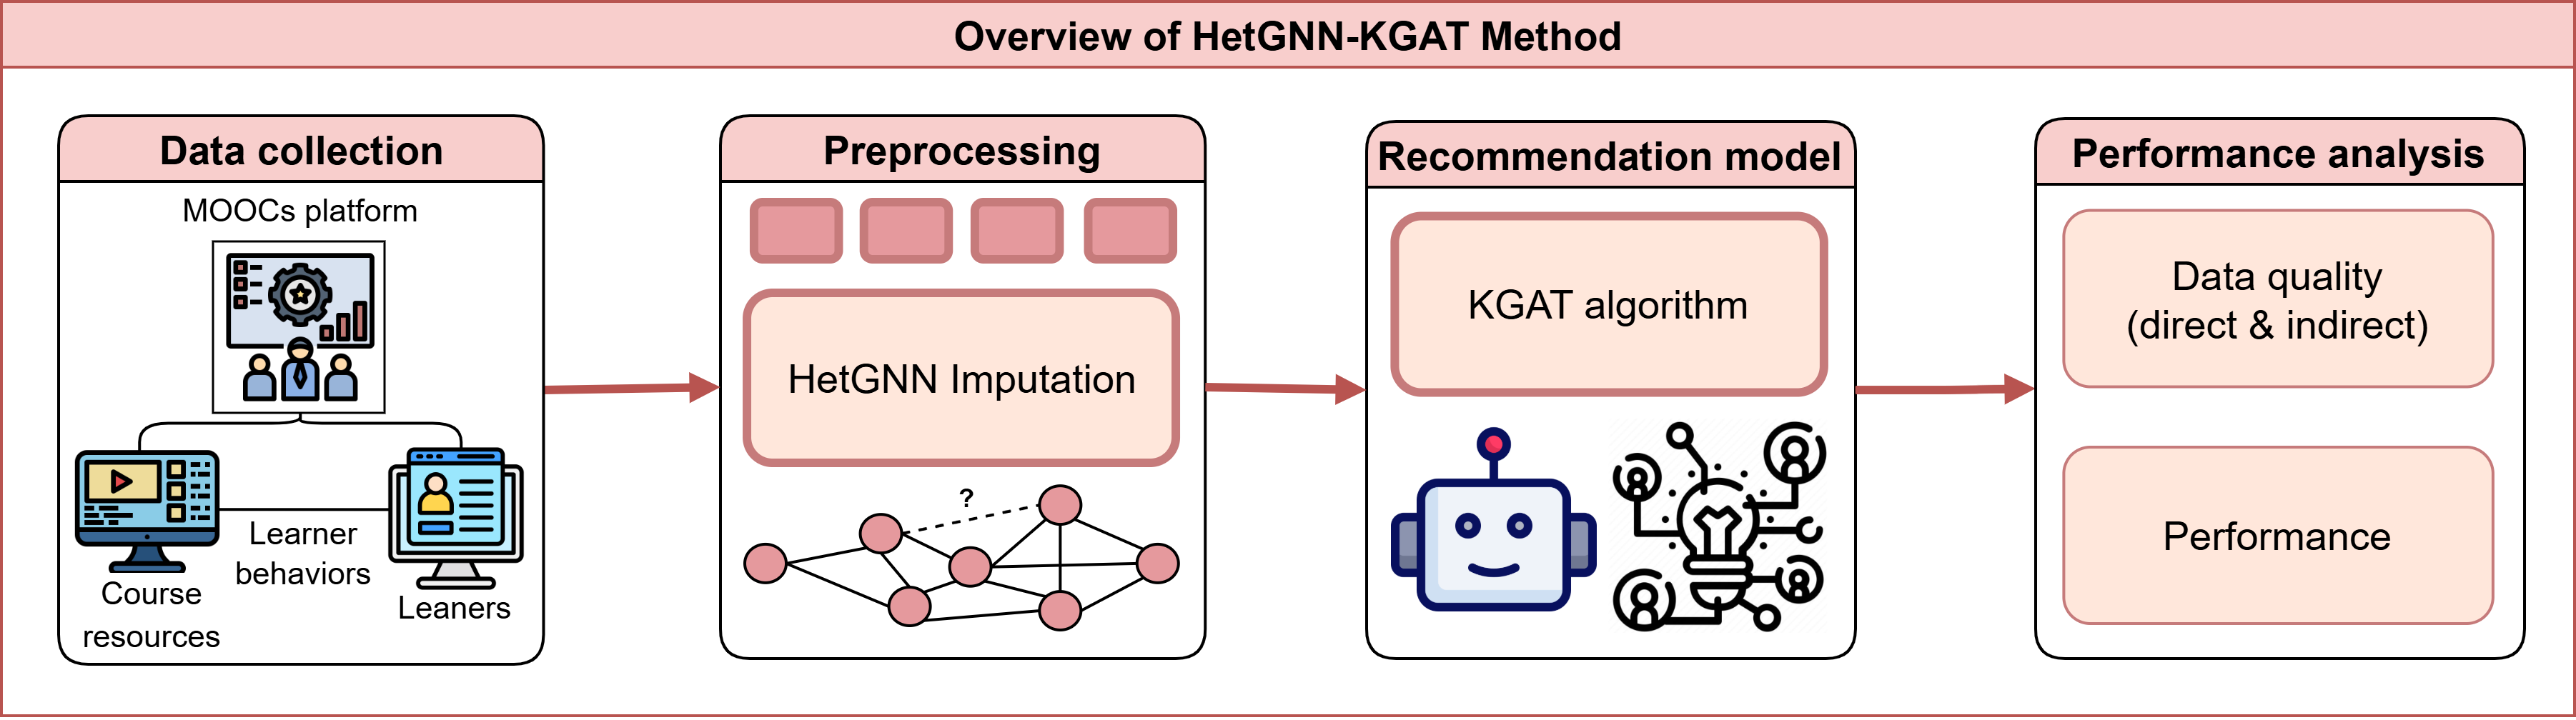
\includegraphics[width=0.8\textwidth]{imgs/overview.png}
\caption{Overview of the HetGNN-KGAT method}
\label{fig:overview_hetgnn_kgat_method}
\end{figure*}

% Presenting evaluation and contributions
Evaluated on the MOOCCubeX dataset, HetGNN-KGAT shows potential improvements in managing sparse data, offering a basis for personalized learning systems. Experimental results demonstrate that HetGNN-KGAT outperforms baseline methods in both simulated and real-world scenarios. On the V5 (HetGNN Imputation) dataset, the proposed method achieves a MAP@10 improvement of 11.85\% to 23.55\% over baselines in simulated settings and 2.83\% to 7.82\% in real-world settings. For V4, V3, and V2 datasets, HetGNN-KGAT consistently surpasses baselines, with improvements ranging from 8.95\% to 20.14\% (simulated) and 2.67\% to 7.92\% (real-world). These results highlight the framework’s ability to enhance data quality and recommendation precision, supporting scalable and adaptive educational systems. Key contributions include an imputation method that performs better than traditional techniques and a recommendation strategy that supports scalability, contributing to future developments in adaptive educational technologies.


The paper is structured as follows. Section~\ref{sec:related_work} reviews related work on recommendation systems, heterogeneous information networks, and MOOC data imputation. Section~\ref{sec:background} presents the theoretical foundations of recommendation systems, graph-based data representation, HetGNN, and KGAT. Section~\ref{sec:proposed_method} details the proposed HetGNN-KGAT framework, including the MOOCCubeX dataset, data analysis, and integration of HetGNN and KGAT. Section~\ref{sec:experiments} evaluates data quality and recommendation performance in simulated and real-world scenarios. Section~\ref{sec:discussion} discusses the method's strengths, limitations, and future directions. Section~\ref{sec:conclusion} summarizes key contributions and implications for personalized learning.

\section{Related Work}
\label{sec:related_work}



\subsection{Missing Data and Imputation Methods}

Handling missing data is essential in MOOCs due to the inherently sparse nature of learner interaction datasets. Various imputation techniques have been explored to improve data quality and mitigate the impact of missing information.

According to the MICE framework \cite{van2011mice}, significant limitations of traditional imputation methods have been highlighted. Specifically, listwise deletion, which removes records with missing values, has been criticized for severely reducing sample size, leading to substantial information loss and diminished statistical power. Meanwhile, simple single imputation methods, such as mean or median imputation, fail to account for the uncertainty associated with missing values, resulting in overly confident but potentially biased statistical estimates.

Troyanskaya et al. (2001) \cite{troyanskaya2001missingDNA} applied machine learning-based approaches, including k-nearest neighbors (k-NN) and Singular Value Decomposition (SVD), to impute missing values in DNA microarray datasets. These methods leverage the similarity among genes or samples to estimate missing entries, producing stable results even under high missing rates. The k-NN approach offers flexibility and is well-suited for multi-dimensional biological data; however, its performance tends to degrade when handling highly nonlinear and complex relationships.

More recently, Graph Neural Networks (GNNs), particularly the HetGNN, have shown outstanding performance in link prediction and missing data imputation tasks on HIN \cite{zhang2019hetgnn}. HetGNN effectively aggregates node content and learns rich, multi-type neighborhood representations, enabling the simultaneous modeling of various entity and relation types. This capability makes HetGNN especially suitable for large-scale and complex datasets like MOOCCubeX, where entities such as learners, courses, videos, and concepts are interconnected through multi-relational structures \cite{yu2021mooccubex}.

The strong link prediction ability of HetGNN offers a promising solution for addressing the pervasive issue of missing data in MOOC systems \cite{kizilcec2015attrition_missing_MOOC}. Additionally, HetGNN’s flexible architecture supports computational optimization, facilitating its deployment in large-scale online education environments. These advantages provide a strong rationale for integrating HetGNN into the proposed HetGNN-KGAT framework, aiming to further enhance input data quality and support more effective personalized course recommendations \cite{zhang2019hetgnn, wang2019kgat}.

\subsection{Recommendation System} 

To help users select suitable content, recommendation systems have been developed using various approaches. Studies are categorized into collaborative filtering, content-based filtering, hybrid, and graph-based methods, each tackling specific challenges in fields like MOOCs.

\subsubsection{Collaborative Filtering}

CF is a key recommendation system technique that leverages user-course interaction data to suggest courses. It includes User-based CF, recommending courses based on similar users' preferences, and Item-based CF, suggesting courses similar to those previously engaged by a user. Despite its accuracy, CF faces cold-start issues with sparse data, common in MOOCs \cite{aggarwal2016recommender}. Bayesian Personalized Ranking (BPR) \cite{rendle2012bprmf} enhances ranking accuracy by 20\% using implicit feedback but struggles with extreme data sparsity \cite{kizilcec2015attrition_missing_MOOC}. Nassar et al.'s (2020) deep neural network-based multi-criteria CF model \cite{nassar2020novel} reduces Mean Absolute Error by 15\% by capturing user behavior, yet it also faces cold-start challenges in sparse MOOC datasets \cite{jordan2014initial_trend_mooc}. CATA++ \cite{alfarhood2020cata++} improves accuracy by 12\% and interpretability using a dual-attention autoencoder but is less scalable for large, heterogeneous MOOC environments \cite{yu2021mooccubex}.

\subsubsection{Content-Based Filtering}

CBF recommends courses by analyzing features of courses and learner profiles, suggesting items with similar characteristics to those a user has enrolled in. Unlike collaborative filtering, CBF is less impacted by sparse data but may limit content discovery due to its reliance on existing user preferences \cite{aggarwal2016recommender}. Science Concierge \cite{achakulvisut2016science}, developed by Achakulvisut et al. (2016), uses Latent Semantic Analysis (LSA) and the Rocchio algorithm, validated on 14,718 papers from the Neuroscience 2015 conference. It outperforms traditional keyword-based methods, offering robust performance in content-rich environments with known user preferences. However, its dependence on existing preferences can lead to repetitive recommendations, failing to meet diverse MOOC learner needs. Additionally, it struggles to capture complex course-learner relationships critical for MOOC platforms \cite{qaffas2020towards, mustafeez2024comprehensive}.

\subsubsection{Hybrid Methods}
Hybrid Recommender Systems combine multiple recommendation techniques to enhance performance, leveraging the strengths of CF and CBF while reducing their individual weaknesses. Common approaches include Weighted Hybrid, which merges scores from different models, Switching Hybrid, which selects the appropriate model per case, and Feature Combination, which uses the output of one model as input for another~\cite{aggarwal2016recommender}. DeepFM~\cite{guo2017deepfm}, a model that integrates Factorization Machines (FM) with deep neural networks (DNNs) for click-through rate (CTR) prediction, was evaluated on advertising datasets and achieved a performance improvement of approximately 15\% compared to traditional baseline methods. DeepFM is capable of jointly learning both low-order (linear) and high-order (nonlinear) feature interactions without requiring manual feature engineering. Despite its effectiveness, the model's performance tends to degrade when dealing with missing or highly complex data structures, such as the irregular and diverse learning behaviors commonly observed in MOOCs~\cite{yu2021mooccubex}. In the context of MOOCs, Li et al. (2023) proposed the Meta Hierarchical Reinforced Ranking (MHRR) model, which achieved over 10\% higher accuracy in course ranking tasks~\cite{li2023mhrr}. While MHRR effectively combines meta-learning and reinforcement signals to optimize hierarchical feedback, its performance declines in real-world MOOC settings due to sparse and noisy interaction data, limiting its scalability and generalizability.

\subsubsection{Graph-Based Recommendation Approaches}
Graph-based models improve MOOC recommendations by capturing complex relationships. Xia et al. (2025) proposed MixRec, using heterogeneous graphs to achieve 60\% accuracy on social datasets, though it struggles with missing data in MOOCs~\cite{xia2025mixrec, kizilcec2015attrition_missing_MOOC}. Nguyen et al. (2024) introduced H-BERT4Rec, combining Heterogeneous Information Networks (HIN) with BERT4Rec for sequential recommendations, achieving 55.04\% accuracy on MOOCCubeX by modeling learner behaviors and multi-relational structures~\cite{nguyen2024hbert4rec, shi2018heterogeneous}. Despite high computational costs and challenges with sparse data, it excels in context-aware personalization. Wang et al. (2019) developed KGAT, integrating collaborative filtering with knowledge graphs, achieving 18\% higher accuracy on Amazon datasets but facing performance issues with sparse MOOC data~\cite{wang2019kgat, yu2021mooccubex}. These insights inform the proposed HetGNN-KGAT framework, which combines heterogeneous graph neural networks and knowledge graph attention to address data sparsity and enhance personalization~\cite{zhang2019hetgnn, wang2019kgat}. Frej et al. (2024) introduced UPGPR, integrating HIN with reinforcement learning to create interpretable learning paths in MOOCs~\cite{frej2024upgpr}. Tested on the MOOCCube dataset, UPGPR leverages HIN to represent diverse relationships and uses reinforcement learning for real-time sequential recommendations, enhancing both personalization and explainability. However, its scalability and performance under sparse MOOC data conditions require further exploration~\cite{kizilcec2015attrition_missing_MOOC}.

\subsection{Heterogeneous Information Networks in Recommender Systems}

To effectively model complex relationships, HIN have been applied in recommender systems. Shi et al. (2018) introduced a HIN embedding approach that utilizes meta-paths, such as "user → item → user", to enhance recommendation performance on the Amazon dataset \cite{shi2018heterogeneous}. This method outperformed traditional homogeneous models by exploiting multi-dimensional relationships among entities. The key advantage of HIN lies in its ability to represent latent connections between different types of entities, making it particularly suitable for MOOC datasets, which typically involve diverse nodes such as learners, courses, and videos.

However, a major limitation of HIN-based methods is their reliance on manually designed meta-paths, which require substantial domain expertise and may not generalize well across datasets. Moreover, their performance tends to degrade when dealing with large-scale datasets or missing data, as commonly observed in MOOCCubeX \cite{yu2021mooccubex}. These challenges highlight the necessity of integrating HIN with other advanced techniques to fully exploit its potential in MOOC recommendation scenarios.

\section{Theoretical Background}
\label{sec:background}

\subsection{Graph-Based Data Representation}

Traditional machine learnings  do not clearly reflect the relationships between objects which is an essential factor in MOOCs, while graph data, where entities are represented as nodes or vertices connected through relationships or edges, allows each node to carry a feature vector and each edge to represent a specific type of relationship between two entities. In the context of MOOCs, graphs enable the modeling of various relationships, such as learners enrolling in courses, courses belonging to specific topics, courses including lectures, learners viewing or completing lectures, and interactions between learners through forums, study groups, or similar platforms. The multidimensional nature and multi-entity characteristics of MOOC data highlight the natural suitability of graph representation, allowing recommendation systems to leverage richer contextual information beyond mere interaction history.

Depending on the data type and application goals, graphs can be categorized into two main types:
\begin{itemize}
    \item Homogeneous Graph: A homogeneous graph is a graph where all nodes and edges are of the same type. For example, in a movie recommendation system, a homogeneous graph might represent users as nodes, with edges connecting users who exhibit similar viewing behaviors. This type is simple and easy to process but does not fully utilize the diversity of entity types and relationships in the data.
    \item Heterogeneous Graph: A heterogeneous graph, also known as a non-homogeneous graph, is a graph where nodes and edges belong to multiple types, reflecting the complex structure of real-world data \cite{shi2018heterogeneous}. In the context of MOOC course recommendation, a heterogeneous graph is used to represent entities such as learners, courses, concepts, teachers, and relationships like enrollment, teaching, or category affiliation. A heterogeneous graph is formally defined as follows:\\
    A heterogeneous graph \( G = (V, E, \phi, \psi) \), where:
    \begin{itemize}
        \item \( V \): set of nodes, where each node \( v \in V \) belongs to a type \( \phi(v) \in \mathcal{A} \), with \( \mathcal{A} \) being the set of node types (e.g., learners, courses).
        \item \( E \): set of edges, where each edge \( e \in E \) belongs to a type \( \psi(e) \in \mathcal{R} \), with \( \mathcal{R} \) being the set of relationship types (e.g., enrollment, teaching).
        \item \( \phi \): node type mapping function, \( \phi: V \rightarrow \mathcal{A} \).
        \item \( \psi \): edge type mapping function, \( \psi: E \rightarrow \mathcal{R} \).
    \end{itemize}

\end{itemize}

Graph data provides several key advantages in MOOC systems. It offers a structured and visual representation, clearly modeling natural connections between educational entities. Additionally, it enables the integration of heterogeneous data, accommodating various entity types and relationships within a single structure. The graph approach is scalable and updatable, allowing easy addition of new nodes, such as new learners or courses, and edges, such as new interactions, without disrupting the system. Furthermore, it serves as a foundation for graph representation learning algorithms, such as GCN, GAT, and R-GCN, which extract informative features for each node to support effective recommendations.

\subsection{Heterogeneous Graph Neural Network}
\label{sec:hetgnn_theory}
GNNs are deep learning models designed to process graph-structured data, where nodes represent entities and edges denote relationships. GNNs generate node embeddings by iteratively aggregating information from a node's neighbors and combining it with its own features, supporting tasks like node classification, link prediction, and recommendation. Variants such as GraphSAGE \cite{hamilton2017inductive} sample neighbors for scalability, while GAT \cite{velivckovic2017graph} employs an attention mechanism to weigh neighbor contributions. 

Building on these principles, Zhang et al. \cite{zhang2019hetgnn} proposed the HetGNN to handle content-associated heterogeneous graphs (C-HetG), which involve multiple node and edge types with diverse content (e.g., text, attributes, images). HetGNN aims to generate node embeddings that capture both heterogeneous structural relationships (e.g., authors writing papers) and varied content attributes, addressing three challenges: sampling correlated heterogeneous neighbors, encoding diverse content, and aggregating information from different neighbor types. To address the first challenge, Zhang et al. \cite{zhang2019hetgnn} employ a random walk with restart strategy to sample a fixed-size set of neighbors for each node \( v \), grouped by type to ensure comprehensive coverage. For content encoding, HetGNN uses a Bi-directional LSTM (Bi-LSTM) to capture interactions among heterogeneous content \( C_v \), producing a content embedding:
\begin{equation}
f_1(v) = \frac{1}{|C_v|} \sum_{i \in C_v} \left[ \overrightarrow{\text{LSTM}}(\mathcal{FC}_{\theta_x}(\mathbf{x}_i)) \oplus \overleftarrow{\text{LSTM}}(\mathcal{FC}_{\theta_x}(\mathbf{x}_i)) \right],
\end{equation}
where \( \mathbf{x}_i \) is a pre-trained feature vector for content item \( i \), \( \mathcal{FC}_{\theta_x} \) is a fully connected layer, and \( \oplus \) denotes concatenation. For neighbor aggregation, HetGNN employs type-specific Bi-LSTMs to aggregate neighbor embeddings, followed by an attention mechanism to combine them with the node's content embedding, yielding the final embedding:
\begin{equation}
\mathcal{E}_v = \alpha^{v,v} f_1(v) + \sum_{t \in \mathcal{A}} \alpha^{v,t} f_2^t(v),
\end{equation}
where \( f_2^t(v) \) is the aggregated embedding for neighbors of type \( t \), and \( \alpha^{v,t} \) are attention weights reflecting the influence of each type. The model is trained end-to-end using a graph context loss with negative sampling, optimizing the objective:
\begin{equation}
o_2 = \sum_{(v, v_c, v_{c'}) \in T_{\text{walk}}} \log \sigma(\mathcal{E}_v \cdot \mathcal{E}_{v_c}) + \log \sigma(-\mathcal{E}_v \cdot \mathcal{E}_{v_{c'}}),
\end{equation}
where \( T_{\text{walk}} \) contains triplets from random walks, and \( v_c, v_{c'} \) are context and negative nodes, respectively. As demonstrated by Zhang et al. \cite{zhang2019hetgnn}, HetGNN excels in tasks like link prediction, recommendation, and node classification, supporting both transductive and inductive learning, though it requires careful hyperparameter tuning and may face computational challenges for large graphs.

\subsection{Knowledge Graph-Based Recommendation Model}

Recommendations powered by knowledge graphs have emerged as a powerful approach to enhance the accuracy and interpretability of recommendation systems. This section delves into the fascinating foundational concepts of these models, drawing significant insights from \cite{wang2019kgat}.

\subsubsection{Knowledge Graph}

A knowledge graph is defined as a heterogeneous network comprising relational triplets between entities, such as (entity: Hugh Jackman, relation: ActorOf, entity: Logan). In recommendation systems, a knowledge graph is integrated with user-item interactions to form a collaborative knowledge graph (CKG). CKG combines a bipartite user-item graph, represented as
\begin{equation}
    G_1 = \{ (u, y_{ui}, i) | u \in U, i \in I\}
\end{equation}
and a knowledge graph, represented as
\begin{equation}
    G_2 = \{ (h, r, t) | h, t \in E, r \in R\}
\end{equation}
Resulting in a comprehensive graph
\begin{equation}
    G = \{ (h, r, t) | h, t \in E' , r \in R' \}
\end{equation}
where \( E' = E \cup U \) (including entities from the KG and users) and \( R' = R \cup \{Interact\} \) (including relations from the KG and interaction relations).

CKG enables modeling of high-order connectivity, i.e., multi-step relational paths between users and items, such as \(
u_1 \xrightarrow{r_1} i_1 \xrightarrow{r_2} e_1 \xrightarrow{r_2} i_2 \xrightarrow{r_1} \{u_2, u_3\}
\). However, directly computing these high-order connections can be computationally intensive, necessitating methods like attention mechanisms to assess the importance of such paths.

Traditional recommendation systems, such as FM, typically treat each user-item interaction as an independent case, with side information encoded. However, this approach fails to leverage relationships between items. For instance, two films may not be directly related but could share a production company or a supporting actor. Knowledge graphs address this limitation by linking items to their attributes, creating a hybrid structure combining a knowledge graph and a user-item graph. Exploring and utilizing these latent connections is key to enhancing recommendation quality. In this structure, high-order relations, connections between items via one or more linked attributes, play a crucial role in improving recommendation performance. Research \cite{wang2019kgat} indicates that using knowledge graphs helps recommendation systems overcome limitations of traditional models, thereby improving prediction accuracy and personalization.

\subsubsection{Attention Mechanism}

KGAT employs an attention mechanism to determine the weights of neighbors during embedding propagation, assessing the importance of high-order relations. The attention score is computed as:
\begin{equation}
\pi(h, r, t) = \left( W_r e_t \right)^\top \tanh \left( W_r e_h + e_r \right)
\end{equation}

This score is then normalized using a softmax function to ensure the total weight sums to 1:
\begin{equation}
\pi(h, r, t) = \frac{\exp(\pi(h, r, t))}{\sum_{(h, r', t') \in N_h} \exp(\pi(h, r', t'))}
\end{equation}

This attention mechanism enables the model to focus on the most relevant information, enhancing interpretability by highlighting influential neighbors or relational paths in recommendations. For example, in a case study on the Amazon-Book dataset, the attention mechanism identified the path \(
u_{208} \xrightarrow{r_0} \text{Old Man's War} \xrightarrow{r_{14}} \text{John Scalzi} \xrightarrow{r_{14}} i_{4293}
\) as having the highest attention score, explaining why item \( i_{4293} \) was recommended to the user \( u_{208} \).

\subsubsection{Embedding Propagation}

Beyond the above theories, the embedding propagation process in KGAT plays a critical role, recursively updating node embeddings based on neighbor information to capture high-order connections. Neighbor information is aggregated as:
\begin{equation}
     e_{N_h} = \sum_{(h, r, t) \in N_h} \pi(h, r, t) e_t
\end{equation}

This process employs aggregation methods such as GCN, GraphSAGE, or Bi-Interaction. For instance, with Bi-Interaction, the aggregation function is defined as:
\begin{equation}
    \begin{split} % Bắt đầu môi trường split
        f_{Bi-Interaction} &= \text{LeakyReLU}(W_1(e_h + e_{N_h})) \\ % Xuống dòng tại đây
        &\quad + \text{LeakyReLU}(W_2(e_h \odot e_{N_h}))
    \end{split} % Kết thúc môi trường split
\end{equation}
Propagation occurs across multiple layers, with the representation at layer \( l \) given by:
\begin{equation}
    e^{(l)}_h = f(e^{(l-1)}_h, e^{(l-1)}_{N_h})
\end{equation}

This allows the model to capture complex relationships, such as \(
u_2 \xrightarrow{r_1} i_2 \xrightarrow{r_2} e_1 \xrightarrow{r_2} i_1 \xrightarrow{r_1} u_1
\). The embedding propagation process has linear time complexity, mitigating computational overhead when handling large graphs.



\section{Proposed Method}
\label{sec:proposed_method}
\subsection{Experimental Data}

MOOCCubeX \cite{yu2021mooccubex} is a comprehensive, knowledge-oriented dataset tailored to advance research in adaptive learning. It encompasses a vast collection of educational resources and learner interactions, including 4,216 courses and 230,263 lecture videos. The dataset also contains 358,265 exercises and 637,572 fine-grained concepts, providing a rich foundation for detailed analysis. Additionally, it captures over 296 million learning behavior records from 3,330,294 learners, offering extensive insights into learner engagement and interactions.

Unlike previous datasets limited by size, detail, or updates, MOOCCubeX provides a rich data structure encompassing course information, instructional content, learner details, learning behaviors, and knowledge relationships. The data is processed and organized with a knowledge-oriented approach through a concept graph extracted from video subtitles using weakly supervised learning models.

\textbf{Course Resources.} Each course hosted on the XuetangX platform is structured into multiple chapters, comprising a sequence of lecture videos and exercises. The collected resource data encompasses comprehensive course information, including the course name, description, instructor details, affiliated university, and classification across 88 academic disciplines. The dataset includes over 2.7 million lecture videos, each accompanied by detailed timeline-based subtitles that facilitate knowledge extraction and behavioral analysis. Additionally, the dataset contains 358,265 exercises, which incorporate over 2.4 million questions categorized into single-choice, multiple-choice, and essay formats.

\textbf{Learner Behaviors.} Learner activities are meticulously documented to provide a granular view of engagement. This includes anonymized learner profiles capturing demographic details such as age, gender, and region. Video-watching behaviors are recorded through over 154 million ``Heartbeat log'' entries, which track viewing activity at five-second intervals. Exercise submissions are represented by over 133 million records, detailing multiple submission attempts, associated scores, and submission timestamps. Furthermore, the dataset includes over 8 million comment and response records tied to specific videos or exercises, reflecting learner interactions within discussion forums.

\textbf{Knowledge Concepts and Prerequisite Relationships.} Through the application of weakly supervised learning and analysis of video subtitles, over 57,000 knowledge concepts have been extracted, alongside the identification of 126,000 prerequisite relationships among these concepts. These concepts are systematically annotated to label videos, exercises, and comments, constructing a HIN. This network serves as a robust foundation for developing knowledge-based recommendation models, enabling advanced analyses and personalized learning experiences.

\subsection{Data Analysis}

To develop and evaluate the HetGNN-KGAT method, the MOOCCubeX dataset is used as the primary data source due to its comprehensiveness and ability to represent entities and complex relationships in the MOOC environment \cite{yu2021mooccubex}. This section describes the selected data files, the data consolidation process, newly created attributes, detailed attribute descriptions, and notable exploratory data analysis (EDA), particularly the missing data rate.

\subsubsection{Data Files Used}

The selected data files from MOOCCubeX include entity and relationship files, listed in Table~\ref{tab:data_files} with their corresponding English names. These files were chosen because they provide essential information for constructing a HIN and supporting the stages of HetGNN-KGAT: relationship representation, data imputation with HetGNN, and recommendation with KGAT \cite{zhang2019hetgnn, shi2018heterogeneous, wang2019kgat}.

\begin{table}[!t]
\centering
\caption{List of data files used from MOOCCubeX}
\label{tab:data_files}
\renewcommand{\arraystretch}{1.2}
\scalebox{0.8}{
\begin{tabular}{|l|l|}
\hline
\textbf{File name} & \textbf{Description} \\
\hline
course.json & Course Information \\
user.json & User Information \\
school.json & School Information \\
teacher.json & Teacher Information \\
video.json & Video Information \\
problem.json & Problem Information \\
concept.json & Concept Information \\
course-field.txt & Course-Field Relation \\
course-school.txt & Course-School Relation \\
course-teacher.txt & Course-Teacher Relation \\
user-video.json & User-Video Interaction \\
exercise-problem.txt & Exercise-Problem Relation \\
user-problem.json & User-Problem Interaction \\
comment-reply.txt & Comment-Reply Relation \\
course-comment.txt & Course-Comment Relation \\
reply-reply.txt & Reply-Reply Relation \\
user-comment.txt & User-Comment Interaction \\
user-reply.txt & User-Reply Interaction \\
video\_id-ccid.txt & Video-Subtitle Relation \\
prerequisites/cs.json & CS Prerequisites \\
prerequisites/math.json & Math Prerequisites \\
prerequisites/psy.json & Psychology Prerequisites \\
\hline
\end{tabular}
}
\end{table}

The selection rationale for the MOOCCubeX dataset encompasses several key components. Entity files, including course.json, user.json, school.json, teacher.json, video.json, problem.json, and concept.json, provide foundational information on essential MOOC entities, which are critical for constructing nodes in a HIN as described in \cite{shi2018heterogeneous}. 
Relationship files, such as course-field.txt, course-school.txt, course-teacher.txt, user-video.json, exercise-problem.txt, user-problem.json, comment-reply.txt, course-comment.txt, reply-reply.txt, user-comment.txt, user-reply.txt, and video\_id-ccid.txt, capture diverse interactions, such as course-field affiliations and learner-video viewing patterns, enabling the exploration of complex data structures as noted in \cite{yu2021mooccubex}. 
Additionally, prerequisite files, including prerequisites/cs.json, prerequisites/math.json, and prerequisites/psy.json, supply prerequisite information for courses in specific academic fields, facilitating structured learning pathways.

\subsubsection{Data Consolidation}

The aforementioned data files are integrated into a unified file comprising 7,284,500 rows and 34 attributes, incorporating newly derived features. The consolidation process involves merging entity and relationship files using primary keys, such as user\_id, course\_id, video\_id, and concept\_id, to ensure data coherence. Data normalization is performed by converting time formats, such as enroll\_time to Unix time, standardizing list structures like \texttt{list<string>} and \texttt{list<float>}, and eliminating invalid entries. Furthermore, new attributes are generated to enrich recommendation capabilities, including course\_total\_comments to reflect total course interactions, user\_course\_num\_comment to track learner comment counts, and user\_course\_num\_replies to capture learner reply counts.
%\subsubsection{Attribute Description}
The attributes of the consolidated data file are detailed in Table~\ref{tab:data_attributes}, including column names, missing data rates, data types, and meanings.

\begin{table}[!t]
\centering
\caption{Description of attributes in the consolidated data file}
\label{tab:data_attributes}
\renewcommand{\arraystretch}{1.2}
\scalebox{0.8}{
\begin{tabular}{|p{3.2cm}|p{1cm}|p{2cm}|p{2.5cm}|}
\hline
\textbf{Column} & \textbf{Missing Rate (\%)} & \textbf{Data type} & \textbf{Description} \\
\hline
user\_id & 0 & string & Learner ID \\
course\_id & 0 & string & Course ID \\
enroll\_time & 0 & int (Unix time) & Course enrollment time \\
course\_name & 0 & string & Course name \\
course\_prerequisites & 0 & string & Course prerequisites \\
course\_about & 0 & string & Course description \\
course\_field & 73.12 & list<string> & Course field \\
school\_id & 0.36 & list<string> & IDs of schools offering the course \\
school\_name & 0.36 & list<string> & Names of schools offering the course \\
school\_about & 0.36 & list<string> & Descriptions of schools offering the course \\
school\_motto & 0.36 & list<string> & Mottos of schools \\
teacher\_id & 0.13 & list<string> & Teacher IDs \\
teacher\_name & 0.13 & list<string> & Teacher names \\
teacher\_about & 0.13 & list<string> & Teacher descriptions \\
teacher\_job\_title & 0.13 & list<string> & Teacher job titles \\
teacher\_org\_name & 0.13 & list<string> & Teacher organizations \\
video\_id & 37.92 & list<string> & Video IDs in the course \\
video\_ccid & 37.92 & list<string> & Video subtitle IDs \\
video\_duration & 37.92 & list<float> & Video durations \\
user\_gender & 0 & int & Learner gender \\
watch\_id & 99.94 & list<string> & Video IDs interacted with by learners \\
total\_watch\_time & 99.94 & list<float> & Total video watching time \\
actual\_watch\_time & 99.94 & list<float> & Actual video watching time \\
exercise\_id & 1.93 & list<string> & Exercise IDs \\
exercise\_num\_problem & 1.93 & list<int> & Number of questions per exercise \\
doing\_exercise\_id & 99.69 & list<string> & IDs of correctly solved exercises \\
doing\_num\_correct & 99.69 & list<int> & Number of correct answers \\
concept\_id & 58.99 & list<string> & Concept IDs \\
concept\_prerequisite & 58.99 & list<string> & Concept prerequisites \\
concept\_name & 58.99 & list<string> & Concept names \\
concept\_field & 58.99 & list<string> & Concept fields \\
course\_total\_comments & 0 & int & Total course interactions \\
user\_course\_num\_comment & 0 & int & Learner comment count \\
user\_course\_num\_replies & 0 & int & Learner reply count \\
\hline
\end{tabular}
}
\end{table}

\subsubsection{Exploratory Data Analysis (EDA)}

EDA was conducted to understand data characteristics and inform the design of the HetGNN-KGAT method. General statistics are presented in Table~\ref{tab:combine_data_overview}, including 7,284,500 rows, 367,103 learners, 2,766 courses, 410 schools, 8,909 teachers, 78 fields, 55,831 videos, 57,303 exercises, and 214,454 concepts.

\begin{table}[!t]
\centering
\caption{Overview of consolidated data}
\label{tab:combine_data_overview}
\renewcommand{\arraystretch}{1.2}
\scalebox{0.8}{
\begin{tabular}{|l|c|}
\hline
\textbf{Metric} & \textbf{Value} \\
\hline
Number of columns & 34 \\
Number of rows & 7,284,500 \\
Number of users & 367,103 \\
Number of courses & 2,766 \\
Number of schools & 410 \\
Number of teachers & 8,909 \\
Number of fields & 78 \\
Number of videos & 55,831 \\
Number of exercises & 57,303 \\
Number of concepts & 214,454 \\
\hline
\end{tabular}
}
\end{table}

Notable analyses of the MOOCCubeX dataset provide critical insights into its structure and utility. The analysis of missing data rates, as depicted in Table~\ref{tab:missing_rate}, reveals significant sparsity in learner interaction attributes. Attributes such as \textit{watch\_id}, \textit{total\_watch\_time}, and \textit{actual\_watch\_time} exhibit a 99.94\% missing rate, while \textit{doing\_exercise\_id} and \textit{doing\_num\_correct} show a 99.69\% missing rate, underscoring the data sparsity common in MOOCs \cite{kizilcec2015attrition_missing_MOOC}.

Further examination of missing data indicates that attributes like \textit{course\_field} (73.12\%) and \textit{concept\_id}, \textit{concept\_prerequisite}, \textit{concept\_name}, and \textit{concept\_field} (58.99\%) also suffer from substantial missing rates. These gaps pose challenges for identifying learning paths. However, core attributes, including \textit{user\_id}, \textit{course\_id}, \textit{course\_name}, \textit{enroll\_time}, \textit{course\_about}, \textit{course\_prerequisites},\\ \textit{course\_total\_comments}, \textit{user\_course\_num\_comment}, and \textit{user\_course\_num\_replies}, demonstrate no missing values, ensuring robust data integrity for constructing HIN \cite{shi2018heterogeneous}.

The entity distribution within MOOCCubeX highlights its knowledge richness. With 214,454 concepts compared to 2,766 courses and 367,103 learners, the dataset is well-suited for advanced models like HetGNN \cite{zhang2019hetgnn}. The learner count, expanded to 367,103 from 24,068 in prior analyses, reflects a significantly larger dataset scale, enhancing the capability to model learner behaviors effectively.
Analysis of learner interactions reveals the value of new attributes such as \textit{course\_total\_comments},\\ \textit{user\_course\_num\_comment}, and \textit{user\_course\_num\_replies}, all with 0\% missing rates. These attributes offer critical insights into social engagement, enabling personalized recommendation systems through models like KGAT \cite{wang2019kgat}.
Finally, the analysis of course fields identifies 78 distinct fields, but the \textit{course\_field} attribute has a 73.12\% missing rate, necessitating advanced imputation methods like those provided by HetGNN to improve data quality \cite{yu2021mooccubex}. Video attributes, including \textit{video\_id}, \textit{video\_ccid}, and \textit{video\_duration}, exhibit a 37.92\% missing rate, indicating persistent challenges in collecting comprehensive course material data.
These analyses provide a foundation for designing the HetGNN-KGAT method, particularly using HetGNN for data imputation and KGAT for course recommendations \cite{zhang2019hetgnn, shi2018heterogeneous, wang2019kgat}.
\subsection{HetGNN-KGAT: Personalized Course Recommendation via Knowledge Graph Completion and Attention-based Modeling}

\begin{table}[h]
    \centering
    \caption{Missing value rate per column in the consolidated dataset}
    \label{tab:missing_rate}
    \scalebox{0.8}{
        \fbox{%
            \begin{tabular}{ccc}
                \toprule
                \textbf{No.} & \textbf{Column Name} & \textbf{Missing Rate (\%)} \\
                \midrule
                1 & actual\_watch\_time & 99.94 \\
                2 & watch\_id & 99.94 \\
                3 & total\_watch\_time & 99.9 \\
                4 & doing\_exercise\_id & 99.69 \\
                5 & doing\_num\_correct & 99.69 \\
                6 & course\_field & 73.12 \\
                7 & concept\_prerequisite & 59.0 \\
                8 & concept\_field & 59.0 \\
                9 & concept\_name & 59.0 \\
                10 & concept\_id & 59.0 \\
                11 & video\_duration & 37.9 \\
                12 & video\_id & 37.9 \\
                13 & video\_ccid & 37.9 \\
                14 & exercise\_jd & 1.9 \\
                15 & exercise\_num\_problem & 0.4 \\
                16 & school\_name & 0.4 \\
                17 & school\_motto & 0.4 \\
                18 & school\_about & 0.4 \\
                19 & school\_id & 0.4 \\
                20 & teacher\_org\_name & 0.1 \\
                21 & teacher\_job\_title & 0.1 \\
                22 & teacher\_id & 0.1 \\
                23 & teacher\_name & 0.1 \\
                24 & teacher\_about & 0.0 \\
                25 & course\_id & 0.0 \\
                26 & user\_id & 0.0 \\
                27 & course\_about & 0.0 \\
                28 & course\_prerequisites & 0.0 \\
                29 & course\_name & 0.0 \\
                30 & enroll\_time & 0.0 \\
                31 & user\_gender & 0.0 \\
                32 & course\_total\_comments & 0.0 \\
                33 & user\_course\_num\_comment & 0.0 \\
                34 & user\_course\_num\_replies & 0.0 \\
                % \bottomrule
            \end{tabular}
        }
    }
\end{table}


\begin{figure*}[!t]
\centering
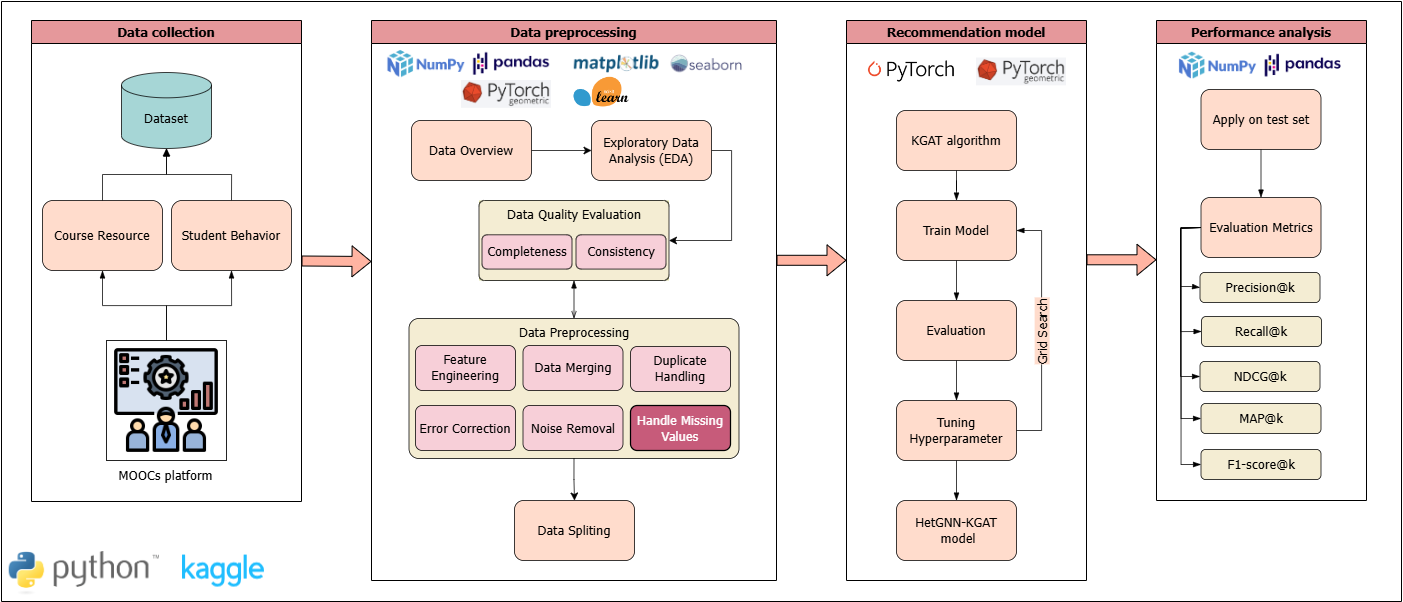
\includegraphics[width=0.9\textwidth]{imgs/framework_journal.png}
\caption{Operational workflow of HetGNN-KGAT}
\label{fig:framework}
\end{figure*}
The proposed recommendation system in this study follows a three-stage process as depicted in Figure~\ref{fig:framework}: data collection and processing, building a combined recommendation model with link prediction, and performance evaluation. The primary goal of the method is not only to recommend suitable courses for learners but also to detect and impute missing links between entities in the MOOC knowledge graph, thereby refining the data structure to support more accurate recommendation inference.

Data is collected from MOOCs, comprising two main components: course resources and learner behaviors. Course resources describe academic information such as titles, descriptions, concepts, instructors, organizing institutions, and subject categories. Meanwhile, learner behaviors record their interaction history, including enrolled courses, completed exercises, or interactions with learning videos. The data is consolidated into a heterogeneous graph where each node represents an entity and each edge represents a relationship between these entities.

After collection, the data undergoes a processing stage to ensure quality before model construction. This stage begins with an overview data analysis and exploratory data mining to identify key features, determine distributions, and detect potential issues. The data is then assessed for completeness and consistency—two factors that directly impact the accuracy of the recommendation model \cite{nguyen2025data_quality}. The preprocessing includes technical operations such as feature extraction, data merging from multiple sources, handling duplicates, noise removal, and, notably, missing value imputation. In the proposed method, imputation of these missing values is handled using a link prediction model based on the HetGNN knowledge graph architecture.

The core of the system is a hybrid recommendation model integrating HetGNN and KGAT. HetGNN is responsible for learning node representations on a heterogeneous graph by leveraging content and neighbor information for each entity to generate semantically rich embeddings. These node representations are subsequently used in a link prediction task to identify missing relationships between entities, particularly between learners and courses. This step is crucial for imputing data in the input graph, enhancing its completeness and improving the effectiveness of the recommendation inference stage. Specifically, predicted links with high probability are added to the knowledge graph as potential relationships, thereby improving the ability to detect accurate paths in the recommendation phase.

After enriching the knowledge graph (CKG) with predicted links, the recommendation model applies KGAT to effectively exploit high-order relationships between learners and courses. KGAT integrates graph neural networks with an attention mechanism, using embedding propagation layers to update representations of entities (learners, courses, attributes) based on information from neighboring nodes. This process enables the model to automatically learn multi-level connections within the CKG, enhancing prediction capabilities without requiring predefined path patterns as in traditional methods.

The entire trained model is evaluated using a separate test dataset, employing metrics such as Precision@k, Recall@k, NDCG@k, and MAP@k as described in \cite{nguyen2024hbert4rec, nguyen2025data_quality} to measure recommendation quality. Evaluation results are used to optimize the model by tuning hyperparameters, ensuring maximum effectiveness for personalized recommendation tasks in online learning environments.

\subsubsection{Implementation of HetGNN for Imputation}
HetGNN is used to impute sparse data by learning node embeddings from a heterogeneous graph, leveraging content and relational structure with two convolution layers (Algorithm \ref{alg:hetgnn}). Its selection for personalized course recommendation in MOOCs addresses data sparsity and complex relationships in the dataset, which limit modeling user preferences and course relevance. HetGNN models MOOCs data as a heterogeneous graph, capturing relationships like user-course interactions and course-concept prerequisites. Unlike Listwise Deletion, which risks information loss, or Statistical Imputation, which may introduce bias, HetGNN preserves data integrity by exploiting content and relational structures. Compared to KNN-based imputation, it better handles complex relationships, ensuring robust data processing. HetGNN enhances input data for the KGAT recommendation model, improving personalization by synthesizing user behavior and course attributes.

\begin{algorithm}
\caption{Two-Layer HetGNN Details}
\label{alg:hetgnn}
\small
\begin{algorithmic}[1]
\Require
    \State $x\_dict$: Dictionary of initial node feature vectors (e.g., text descriptions, numerical data).
    \State $edge\_index\_dict$: Dictionary of edge indices for each relationship type in the heterogeneous graph.
    \State $metadata[1]$: List of edge types in the heterogeneous graph.
    \State $hidden\_channels = 32$: Size of hidden vector space.
\Ensure
    \State $x\_dict$: Dictionary of final node representation vectors.
\State \textbf{Initialize} HetGNN model with $hidden\_channels = 32$.
\State \textbf{Input Layer}:
    \State Receive $x\_dict$ (node features) and $edge\_index\_dict$ (graph structure).
\State \textbf{Convolution Layer 1 (conv1)}:
    \State Apply $HeteroConv$ with $SAGEConv$ modules for each $edge\_type \in metadata[1]$.
    \State Map node features from initial space ($-1$) to hidden space ($hidden\_channels = 32$).
    \State Aggregate neighbor features using $aggr=sum$ for each edge type.
    \State Obtain node representation vectors after first convolution.
\State \textbf{Activation}:
    \State Apply $relu$ function to each node vector, preserving $None$ values if present.
\State \textbf{Convolution Layer 2 (conv2)}:
    \State Apply another $HeteroConv$ layer with $SAGEConv$ modules, using output vectors from $conv1$.
    \State Aggregate neighbor features using $aggr=sum$ for each edge type.
    \State Obtain refined node representation vectors.
\State \textbf{Output}:
    \State Return $x\_dict$, containing final node representation vectors.
\State \textbf{Application}:
    \State Use output vectors to impute sparse data or as input for KGAT.
\end{algorithmic}
\end{algorithm}

{The HetGNN algorithm operates through a structured process to generate node embeddings. Initially, it takes node features (e.g., course descriptions, user profiles) and the graph's relational structure as input. It then samples a fixed set of neighboring nodes for each entity using a random walk strategy, grouping them by type to capture diverse relationships. These neighbors' features are encoded using a neural network to form initial embeddings. In the first convolution layer, the logic aggregates information from these neighbors for each relationship type, combining it with the node's own features. A non-linear activation function is applied to refine these embeddings. The second convolution layer repeats this aggregation to capture deeper interactions, producing final node embeddings. These embeddings are used to impute missing data, enhancing the quality of input for the recommendation model. This two-layer architecture ensures HetGNN can learn deep representations, combining heterogeneous neighbor information, and efficiently handle sparse data by aggregating across relationship types.}

\subsubsection{ Implementation of KGAT for Recommendation}
{The KGAT model \cite{wang2019kgat} is selected for implementation in the proposed method to generate course recommendations for users on data enriched by HetGNN. The HetGNN-KGAT implementation process follows the procedure outlined below (Figure \ref{fig:details_of_KGAT}). The selection of KGAT for personalized course recommendation in MOOCs is motivated by its ability to address the challenges of data sparsity and the complex relationships inherent in the MOOCs dataset. These challenges limit the ability to model user preferences and course relevance effectively, necessitating a method that can exploit intricate relational structures.}

{KGAT is designed to leverage knowledge graphs by modeling high-order relationships among entities (e.g., users, courses, concepts) through a collaborative filtering approach enhanced with an attention mechanism. This makes it well-suited for MOOCs data, which includes diverse entities and relationships such as user-course interactions and course-concept prerequisites, organized as a heterogeneous graph. Unlike CBF, which relies solely on course content and overlooks relational context, KGAT captures multi-hop connections (e.g., user \(\rightarrow\) course \(\rightarrow\) concept \(\rightarrow\) related course) to enhance recommendation relevance. Compared to models like DeepFM, which do not explicitly utilize graph structures, or BPRMF, which depends on implicit feedback without considering high-order relationships, KGAT prioritizes significant relationships through its attention mechanism, improving personalization. Additionally, KGAT’s computational efficiency makes it suitable for large-scale MOOCs data, unlike reinforcement learning-based approaches such as UPGPR, which may incur high computational costs. By integrating with HetGNN’s enriched data, KGAT effectively utilizes high-quality node embeddings to produce accurate and personalized course recommendations, addressing the need for synthesizing user behavior and course attributes in the MOOCs recommendation problem.
}

\paragraph{Construction of a Knowledge Graph in the MOOC Context}

The construction process inherently begins with the precise identification of the graph's fundamental components: nodes and edges. Within the MOOC data landscape, nodes typically represent key entities such as users, courses, schools, teachers, fields of study, videos, and concepts. Following the definition of nodes, a critical task is to delineate the diverse relationships (edges) that interconnect these entities. For instance, a user enrolls in a course, a course is taught by a teacher, a course is offered by a school, a course belongs to a specific field, a course contains video lectures, and these videos convey particular concepts. The meticulous identification and structuring of these entities and their interrelations form the bedrock for constructing a comprehensive Collaborative Knowledge Graph (CKG).

\paragraph{Training the KGAT Model on the Constructed Graph Data}

Represent nodes (users, courses, entities) in the knowledge graph as embedding vectors, forming the foundation for subsequent steps. Use TransR, a translation-based embedding method, ensuring that the embedding vectors of the relation \( r \) and head \( h \), tail \( t \) nodes comply with:
\begin{equation}
    e_r^h + e_r \approx e_r^t
\end{equation}

Where \( e_r^h \), \( e_r \), \( e_r^t \) are the corresponding embedding vectors.

The feasibility score is calculated as:
\begin{equation}
    g(h, r, t) = \|W_r e_h + e_r - W_r e_t\|_2^2
\end{equation}

Where \( W_r \) is a relation-specific matrix that maps vectors into an appropriate space.

Employ pairwise ranking loss to optimize the knowledge graph:
\begin{equation}
    L_{KG} = \sum_{(h, r, t, t') \in T} -\ln \sigma(g(h, r, t') - g(h, r, t))
\end{equation}

Where \( T = \{(h, r, t, t') | (h, r, t) \in G, (h, r, t') \notin G\} \), and \( G \) is the set of triples in the knowledge graph.

Propagate information from a node’s neighbors to update representations while modeling high-order relationships through an attention mechanism. Subsequently, use aggregators to combine node and neighbor representations. This is performed recursively over \( L \) layers, with the representation at layer \( l \) updated as:
\begin{equation}
    e_h^{(l)} = f(e_h^{(l-1)}, e_{N_h}^{(l-1)})
\end{equation}
Where \( e_{N_h}^{(l-1)} = \sum_{(h, r, t) \in N_h} \pi(h, r, t) e_t^{(l-1)} \).
From the updated representations, predict the interaction probability between user \( u \) and course \( c \).

Combine representations from all propagation layers:
\begin{equation}
    e_u^* = e_u^{(0)} || \cdots || e_u^{(L)}, \quad e_i^* = e_i^{(0)} || \cdots || e_i^{(L)}
\end{equation}

Where \( || \) denotes vector concatenation, producing a longer composite vector.

Use the inner product to compute the score:
\begin{equation}
    \hat{y}(u, i) = e_u^{*\top} e_i^*
\end{equation}
This value represents the compatibility level between user \( u \) and course \( c \).

KGAT employs two primary loss components: the Collaborative Filtering Loss, formulated using Bayesian Personalized Ranking (BPR) loss:
\begin{equation}
    L_{CF} = \sum_{(u, i, j) \in O} -\ln \sigma(\hat{y}(u, i) - \hat{y}(u, j))
\end{equation}
Where \( O = \{(u, i, j) | (u, i) \in I, (u, j) \notin I\} \), and \( I \) is the set of known user-item interactions.
And \( L_{KG} \) to compute the total loss function:
\begin{equation}
    L_{KGAT} = L_{KG} + L_{CF} + \lambda \| \Theta \|_2^2
\end{equation}
Where \( \Theta = \{E, W_r, \forall r \in R, W_1^{(l)}, W_2^{(l)}, \forall l \in \{1, \cdots, L\}\} \) is the set of parameters, and \( \lambda \) is the regularization coefficient.

Additionally, mini-batch Adam with alternating optimization is used to ensure efficient training on large datasets.
\begin{figure*}[!t]
\centering
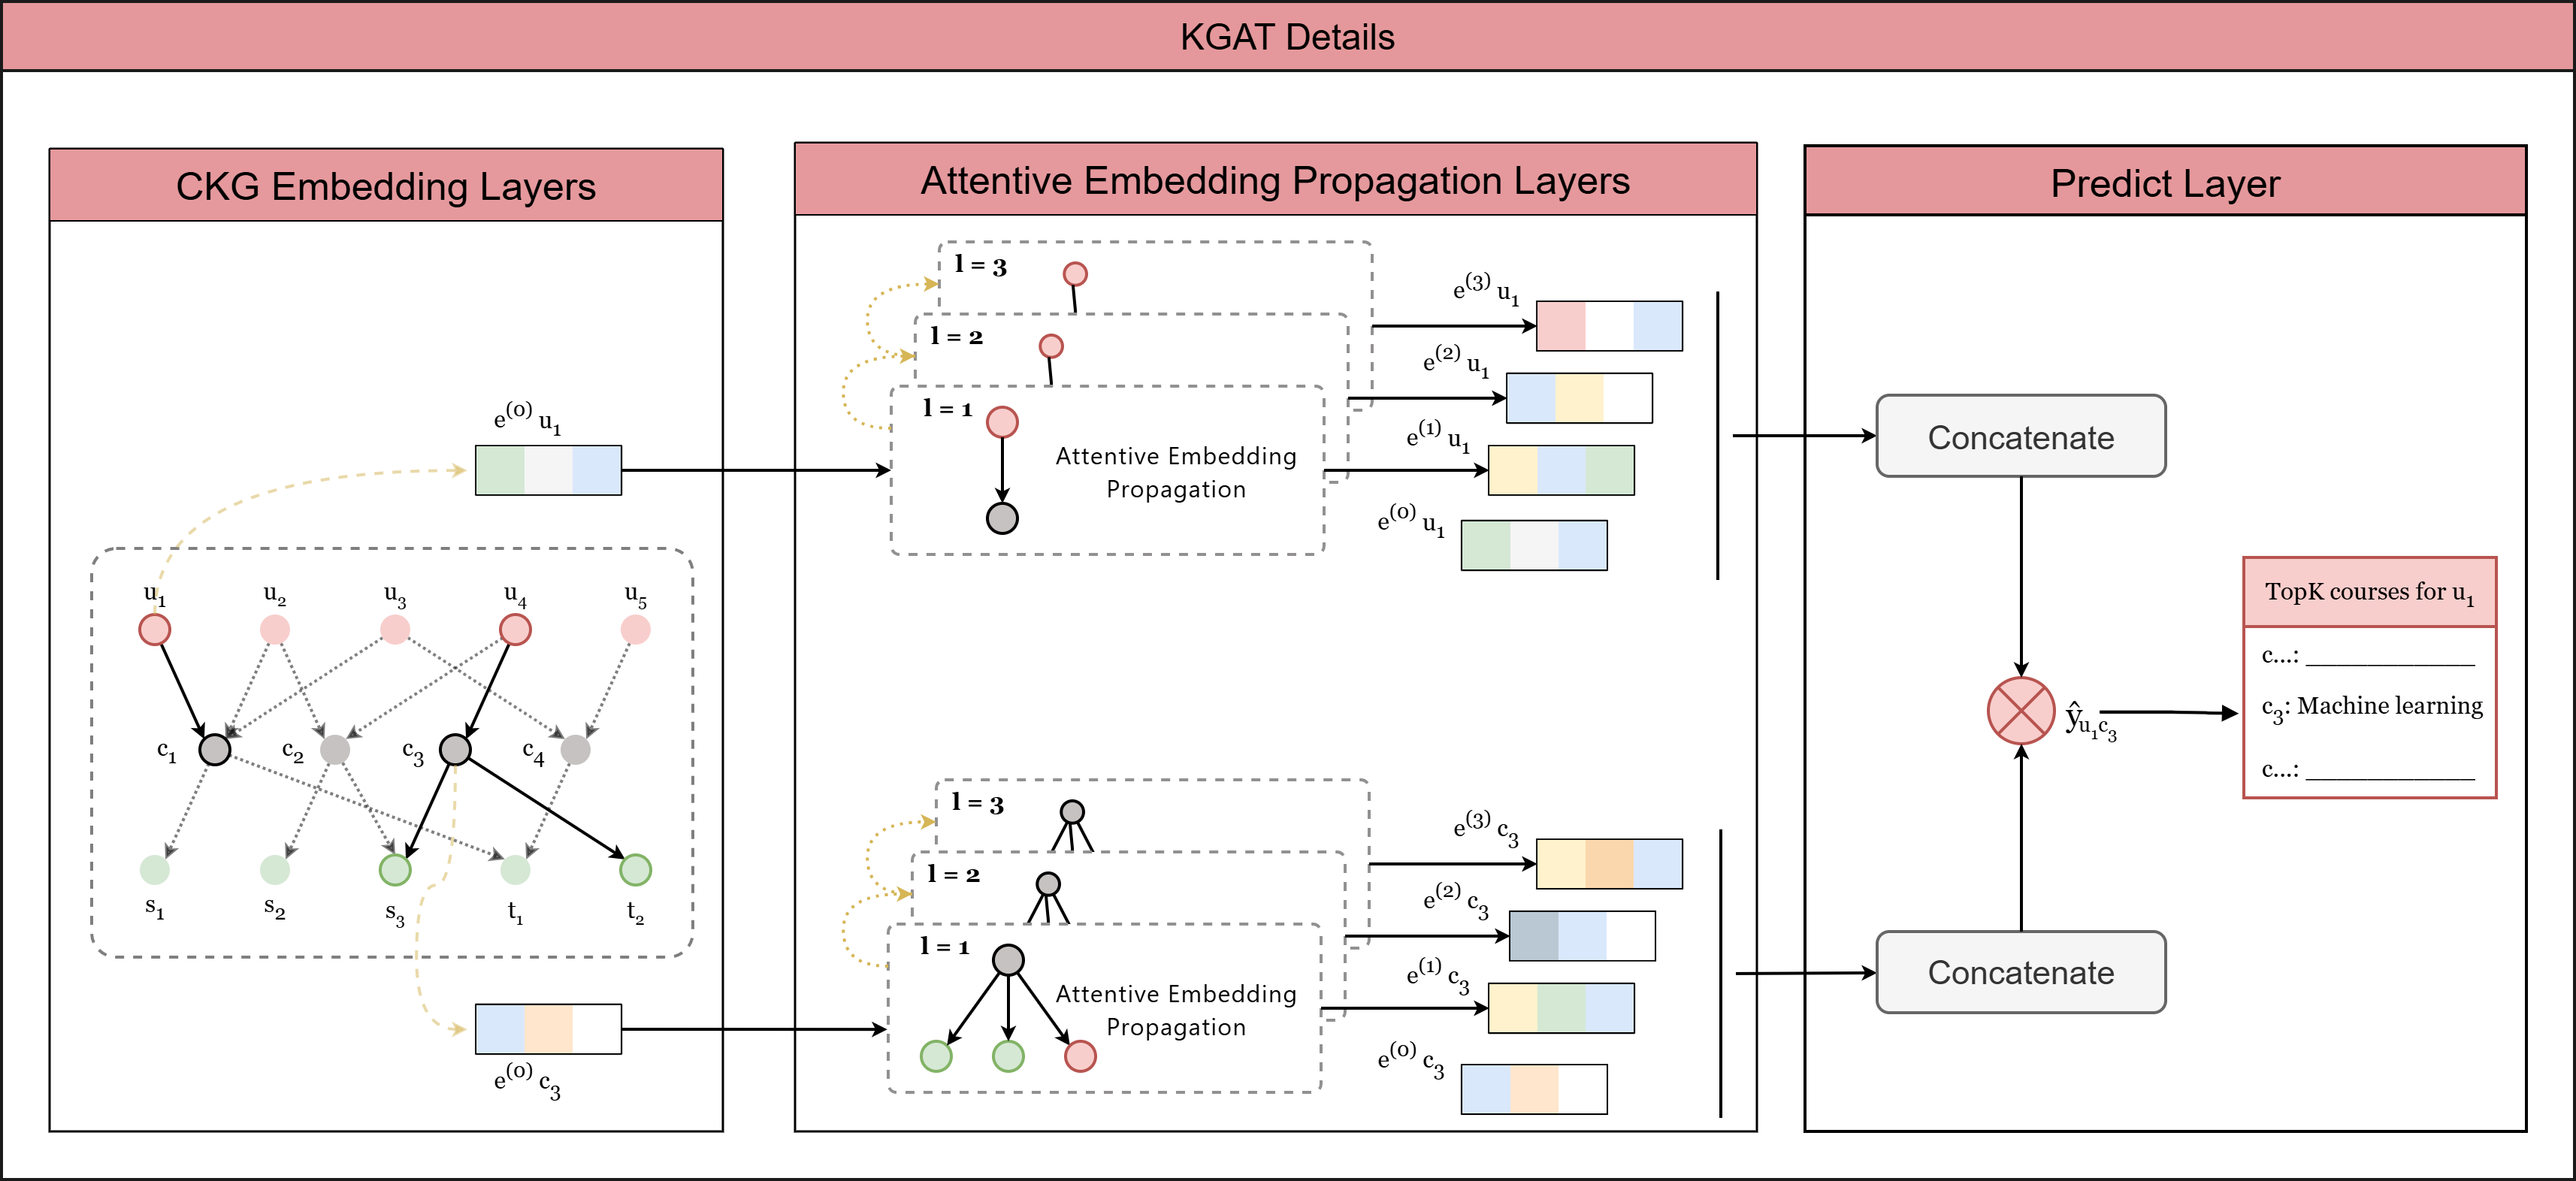
\includegraphics[width=2\columnwidth]{imgs/details_of_KGAT.png}
\caption{Details architecture of KGAT}
\label{fig:details_of_KGAT}
\end{figure*}


\section{Experiments}
\label{sec:experiments}

The source code, datasets, and supplementary materials of this study are available on GitHub HetGNN-KGAT-for-EduPath \footnote{ \url{https://github.com/datachain-uit/HetGNN-KGAT-for-EduPath}}

\subsection{Evaluation Metrics}

To comprehensively assess both the quality of the input data and the effectiveness of the recommendation models, we group the evaluation metrics into three categories: \textit{Direct Data Quality Metrics}, \textit{Indirect Data Quality Metrics}, and \textit{Overall System Performance}.

\subsubsection{Direct Data Quality Metrics}
\label{subsubsec:direct DQ}
The quality of the input data is a critical factor influencing the effectiveness of machine learning models. To quantify the cleanliness, completeness, and validity of the dataset before training the recommendation model, we use two direct data quality metrics: completeness and consistency \cite{nguyen2025data_quality}.

\paragraph*{Completeness}

The completeness metric \cite{nguyen2025data_quality} reflects the extent of data completeness, specifically the proportion of non-missing values across the entire dataset. A higher completeness value indicates less missing data, thereby increasing the reliability of model training.

Defining completeness for a single object:
\begin{equation}
    \text{Completeness}_{\text{object}} = \frac{|\{a_i \in A \mid a_i \neq \text{NaN} \land a_i \neq \text{None}\}|}{|A|}
\end{equation}

\begin{itemize}
    \item \( A = \{a_1, a_2, \ldots, a_n\} \) is the set containing all values of an object.
    \item \( a_i \) is the value of the \( i \)-th attribute.
    \item \( |A| \) is the total number of attributes.
    \item The numerator counts the number of attributes that are neither \(\text{NaN}\) nor \(\text{None}\).
\end{itemize}

Defining completeness for the entire dataset as the average completeness across all objects over \( N \) total objects:
\begin{equation}
\text{Completeness}_{\text{dataset}} = \frac{1}{N} \sum_{j=1}^{N} \text{Completeness}_{\text{object}_j}
\end{equation}


\paragraph*{Consistency}

The consistency metric \cite{nguyen2025data_quality} measures the extent to which the data adheres to predefined validity rules. A record is considered "valid" if it violates none of the validation rules from the following groups: value domain, non-null data, data type, logical constraints, uniqueness, and foreign key integrity.

Defining consistency for a single object:
\begin{equation}
\text{Consistency}_{\text{object}} = \frac{|\{c_j \in C \mid \text{isValid}(c_j) = \text{True}\}|}{|C|}
\end{equation}


\begin{itemize}
    \item \( C = \{c_1, c_2, \ldots, c_m\} \) is the set containing all constraints applied to an object.
    \item \(\text{isValid}(c_j)\) is a function that checks the constraint \( c_j \) on the object (returns \(\text{True}\) if the constraint holds).
    \item \( |C| \) is the total number of constraints.
\end{itemize}

Types of constraints:
\begin{itemize}
    \item Domain Range: \( a_i \in [v_{\text{min}}, v_{\text{max}}] \)
    \item Non-null: \( a_i \neq \text{null} \)
    \item Data Type: \( a_i \in \text{type}(a_i) \)
    \item Logical Constraints: \( a_i \) satisfies the logical condition \( a_i > a_j \)
    \item Uniqueness: \( a_i \notin \text{duplicates}(A) \)
    \item Foreign Key Integrity: \( a_i \in \text{ReferenceTable} \)
\end{itemize}

Defining consistency for the entire dataset as the average consistency across all objects over \( N \) total objects:
\begin{equation}
\text{Consistency}_{\text{dataset}} = \frac{1}{N} \sum_{j=1}^{N} \text{Consistency}_{\text{object}_j}
\end{equation}

Specific validation criteria are described as follows:\\
Domain Range: Values must fall within specified ranges or sets to ensure data validity.

\begin{itemize}
    \item Column \textit{user\_gender} belongs to the set \{0, 1, 2\}.
    \item \textit{user\_id} starts with "U\_", \textit{course\_id} starts with "C\_".
    \item \textit{enroll\_time} $\in [2019, 2020]$ (within the data collection timeframe).
    \item Columns: \textit{total\_course\_comments},\linebreak \textit{user\_course\_num\_comment}, \textit{user\_course\_num\_replies} must be non-negative integers ($\ge 0$).
    \item Columns in list format such as: \textit{num\_problem}, \textit{num\_correct\_problem}, \textit{video\_duration}, \linebreak\textit{actual\_watch\_time}, \textit{total\_watch\_time} are lists of non-negative numbers.
\end{itemize}

Non-null Data: Essential columns must have values to ensure completeness of critical data.
\begin{itemize}
    \item \textit{user\_id}, \textit{course\_id}, \textit{school\_id}, \textit{teacher\_id}, \textit{course\_field} must not be empty.
\end{itemize}

Data Type: Data must conform to specified types to ensure proper processing and analysis.
\begin{itemize}
    \item \textit{enroll\_time}: Unix timestamp (int) type.
    \item \textit{user\_gender}, \textit{total\_course\_comments}, \\\textit{user\_course\_num\_comment}, \textit{user\_course\_num\_replies}: int type.
    \item \textit{user\_id}, \textit{course\_id}, \textit{course\_name}, \textit{course\_prerequisites}, \textit{course\_about}: string type.
    \item Fields like \textit{school\_id}, \textit{teacher\_id}, \textit{video\_id}, \textit{ccid}, \textit{watch\_id}, \textit{exercise\_id}, \textit{concept\_id}, \textit{concept\_prerequisite}, \dots: list type of strings.
\end{itemize}

Logical Constraints: Data must satisfy logical rules to maintain coherence and correctness.
\begin{itemize}
    \item \textit{actual\_watch\_time} $\le$ \textit{total\_watch\_time}.
    \item \textit{actual\_watch\_time} $\le$ \textit{video\_duration}.
    \item \textit{user\_course\_num\_comment} + \textit{user\_course\_num\_replies} $\le$ \textit{total\_course\_comments}.
    \item Each \textit{concept\_id} must not be in its corresponding \textit{concept\_prerequisite} list (avoiding loops).
    \item \textit{num\_correct\_problem} $\le$ \textit{num\_problem}.
\end{itemize}

Uniqueness: Data entries must be unique to prevent duplication and ensure data integrity.
\begin{itemize}
    \item The pair (\textit{user\_id}, \textit{course\_id}) is unique in the dataset ensuring a learner does not appear twice with the same course.
    \item Check for duplicate records: both with all attributes and excluding primary keys (\textit{user\_id}, \textit{course\_id}).
\end{itemize}

Foreign Key Integrity: Each value in the ID columns must exist in the original MOOCCubeX data files:

\begin{table}[H]
\centering
\caption{Foreign key validation with MOOCCubeX entity files}
\scalebox{0.75}{
\begin{tabular}{|l|l|l|}
\hline
\textbf{Column in dataset} & \textbf{Reference file} & \textbf{Notes} \\
\hline
\texttt{user\_id} & \texttt{user.json} & List of learners \\
\texttt{course\_id} & \texttt{course.json} & List of courses \\
\texttt{school\_id} & \texttt{school.json} & Schools offering courses \\
\texttt{teacher\_id} & \texttt{teacher.json} & Instructors teaching courses \\
\texttt{concept\_id} & \texttt{concept.json} & Set of knowledge concepts \\
\texttt{exercise\_id} & \texttt{exercise-problem.json} & Set of exercises \\
\texttt{ccid} & \texttt{video\_id-ccid.txt} & Mapping between videos and concepts \\
\hline
\end{tabular}
}
\end{table}

\subsubsection{Indirect Data Quality Metrics}

The quality of data can be indirectly assessed through the performance effectiveness of machine learning models utilizing that data. In the context of recommendation systems, the following metrics reflect the reliability and relevance of recommendation outcomes when input data is processed using different preproccessing strategies similar to \cite{nguyen2025data_quality, nguyen2024hbert4rec}.

\paragraph*{Reliability}

The reliability of recommendation results is measured using the Mean Average Precision (MAP) metric, which reflects the overall ranking accuracy across all users.

For each user \( u \in U \), Average Precision (AP) is defined as:

\begin{equation}
AP_u = \frac{1}{|R_u|} \sum_{k=1}^{N} P@k \cdot \mathbb{I}(r_k \in R_u)
\end{equation}

Where:
\begin{itemize}
    \item \( R_u \) is the set of correct target items to recommend for user \( u \),
    \item \( r_k \) is the recommended item at position \( k \),
    \item \( P@k \) is the precision at position \( k \),
    \item \( \mathbb{I}(\cdot) \) is an indicator function, equal to 1 if true, 0 if false.
\end{itemize}

The MAP value across all users is calculated as:

\begin{equation}
MAP = \frac{1}{|U|} \sum_{u \in U} AP_u
\end{equation}

\paragraph*{Relevance}

The relevance of recommended items is measured using three common metrics:

\begin{itemize}
    \item Precision@K: The proportion of recommended items within the top-$K$ that are correct:

    \begin{equation}
    Precision@K = \frac{|R_u \cap \hat{R}_u^K|}{K}
    \end{equation}

    \item Recall@K: The proportion of correct items recommended by the model:

    \begin{equation}
    Recall@K = \frac{|R_u \cap \hat{R}_u^K|}{|R_u|}
    \end{equation}

    \item Normalized Discounted Cumulative Gain (NDCG@K): Considers the position of correct items in the recommendation list. Specifically, NDCG at position \( K \) is calculated as:

    \begin{equation}
    NDCG@K = \frac{DCG@K}{IDCG@K}
    \end{equation}

    Where:
    \begin{equation}
    DCG@K = \sum_{i=1}^{K} \frac{rel_i}{\log_2(i + 1)},
    \end{equation}
    \(IDCG@K = \text{ideal DCG value with the optimal order}\)

    with \( rel_i \in \{0,1\} \) being the binary relevance of the item at position \( i \).
\end{itemize}

These metrics are computed with \( K = 5 \) and \( K = 10 \) to evaluate effectiveness in realistic top-$K$ recommendation scenarios.

\subsubsection{Overall System Performance}

To concisely and comprehensively summarize the accuracy of the recommendation system, we use the F1-score metric—the harmonic mean of Precision and Recall:

\begin{equation}
F1 = 2 \cdot \frac{Precision \cdot Recall}{Precision + Recall}
\end{equation}

The F1-score balances coverage and precision, making it particularly useful in cases of uneven data distribution or when evaluating the model’s ability to recommend important items without missing too many correct targets.

\subsection{Experimental Methodology}

\subsubsection{Experimental Objectives}

The objective of the experimental section is to evaluate the effectiveness of the proposed HetGNN-KGAT method in handling sparse data and providing recommendations on the MOOCCubeX dataset \cite{yu2021mooccubex}. The experiments focus on:
\begin{itemize}
    \item Comparing the effectiveness of four imputation strategies (listwise deletion, statistical imputation, machine learning-based imputation with KNN, and \textbf{HetGNN}) in improving data quality.
    \item Evaluating the performance of five recommendation models (CBF, DeepFM, BPRMF, UPGPR, \textbf{KGAT}) on imputed data.
    \item Assessing the performance of recommendation models in simulated scenarios with limited test data and real-world scenarios.
\end{itemize}
The experiments are designed with a combination of imputation strategies, recommendation models, and evaluation strategies to thoroughly explore the effectiveness of HetGNN-KGAT, as detailed in Table \ref{tab:preprocessing_baseline_models}.

\subsubsection{Experimental Data}

The experiments focus on the MOOCCubeX dataset \cite{yu2021mooccubex}, a rich dataset from the XuetangX online learning platform, with detailed descriptions provided in Section \ref{sec:proposed_method}. Due to computational resource limitations and to focus on meaningful data, we applied a targeted filtering process as follows: first, selecting courses with video or exercise resources; next, removing experimental courses; then retaining only learners who actively interacted with resources, excluding those with excessively high enrollment counts; and finally keeping only courses and learners with at least five connections. The resulting filtered dataset comprises approximately 335,587 interactions from 24,068 learners and 2,539 courses, with 34 attributes describing learner behaviors, course content, platform context, and temporal characteristics, as shown in Table \ref{tab:filtered_data_overview}.

\begin{table}[H]
\centering
\caption{Overview of the filtered dataset}
\label{tab:filtered_data_overview}
\renewcommand{\arraystretch}{1.2}
\scalebox{0.8}{
\begin{tabular}{|l|c|}
\hline
\textbf{Metric} & \textbf{Value} \\
\hline
Number of columns & 34 \\
Number of rows & 335,587 \\
Number of users & 24,068 \\
Number of courses & 2,539 \\
Number of schools & 398 \\
Number of teachers & 8,454 \\
Number of fields & 77 \\
Number of videos & 54,972 \\
Number of exercises & 53,311 \\
Number of concepts & 214,057 \\
\hline
\end{tabular}
}
% \vspace{-2.2em}
\end{table}

The data is split using a leave-one-out temporal splitting strategy \cite{he2017neural}, where:
the training set includes all prior course interactions for each learner;
the test set contains the latest course interaction for each learner, reflecting a realistic sequential recommendation context \cite{kang2018self_attentive, tang2018personalized}.
This approach ensures temporal order preservation, accurately simulating dynamic real-world recommendation scenarios.

\subsubsection{Imputation Strategies}

Four strategies are applied to handle sparse data in MOOCCubeX:

Listwise Deletion: Removes columns with a missing rate above 50\%, followed by deleting rows containing null values. This method retains clean data but may significantly reduce dataset size.

Statistical Imputation: Replaces missing values with the mean for numerical columns (e.g., \textit{total\_watch\_time}) and the mode for categorical columns (e.g., \textit{course\_field}). This approach is simple but may introduce bias if data is unevenly distributed.

Machine Learning-based Imputation (KNN): Utilizes the K-Nearest Neighbors (KNN) algorithm based on cosine similarity \cite{troyanskaya2001missingDNA}. The process includes:
        \begin{itemize}
            \item Natural Language Processing (NLP) with tokenization and lemmatization using tools like NLTK for text data (e.g., course descriptions).
            \item Encoding data into feature embeddings using the Sentence Transformer model.
            \item Predicting missing values based on the nearest neighbors (k=3) using cosine distance.
        \end{itemize}
        This method leverages semantic relationships, making it suitable for complex data like MOOCCubeX.
        
HetGNN: As described in Section \ref{sec:proposed_method}, HetGNN is implemented with two convolution layers to learn node representations from a heterogeneous graph, imputing missing relationships and attributes based on neighbor and content information.

\subsubsection{Baseline Models and Detailed Implementation}

\begin{table}[H]
\centering
\caption{Preprocessing strategies and baseline models}
\label{tab:preprocessing_baseline_models}
\renewcommand{\arraystretch}{1.1}
\footnotesize
\scalebox{0.7}{ 
\begin{tabular}{lllllccccc}
\hline
\multicolumn{1}{|l|}{\multirow{2}{*}{}} & \multicolumn{4}{c|}{\textbf{Preprocessing}} & \multicolumn{5}{c|}{\textbf{Model}} \\ \cline{2-10}
\multicolumn{1}{|l|}{} & \multicolumn{1}{c|}{\begin{tabular}[c]{@{}c@{}}LD\\ \cite{Rubin2019statistical_analysis_missing_data}\end{tabular}} & \multicolumn{1}{c|}{\begin{tabular}[c]{@{}c@{}}SI\\ \cite{van2011mice}\end{tabular}} & \multicolumn{1}{c|}{\begin{tabular}[c]{@{}c@{}}MLI\\ \cite{troyanskaya2001missingDNA}\end{tabular}} & \multicolumn{1}{c|}{\begin{tabular}[c]{@{}c@{}}HetGNN\\ \cite{zhang2019hetgnn}\end{tabular}} & \multicolumn{1}{c|}{\begin{tabular}[c]{@{}c@{}}CBF\\ \cite{achakulvisut2016science}\end{tabular}} & \multicolumn{1}{c|}{\begin{tabular}[c]{@{}c@{}}DeepFM\\ \cite{guo2017deepfm}\end{tabular}} & \multicolumn{1}{c|}{\begin{tabular}[c]{@{}c@{}}BPRMF\\ \cite{rendle2012bprmf}\end{tabular}} & \begin{tabular}[c]{@{}c@{}}UPGPR\\ \cite{frej2024upgpr}\end{tabular} & \multicolumn{1}{c|}{\begin{tabular}[c]{@{}c@{}}KGAT\\ \cite{wang2019kgat}\end{tabular}} \\ \hline
\multicolumn{1}{|c|}{RM-1} & \multicolumn{1}{c|}{$\checkmark$} & \multicolumn{1}{l|}{} & \multicolumn{1}{l|}{} & \multicolumn{1}{l|}{} & \multicolumn{1}{c|}{$\checkmark$} & \multicolumn{1}{c|}{$\checkmark$} & \multicolumn{1}{c|}{$\checkmark$} & \multicolumn{1}{c|}{$\checkmark$} & \multicolumn{1}{c|}{$\checkmark$} \\ \hline
\multicolumn{1}{|c|}{RM-2} & \multicolumn{1}{l|}{} & \multicolumn{1}{c|}{$\checkmark$} & \multicolumn{1}{l|}{} & \multicolumn{1}{l|}{} & \multicolumn{1}{c|}{$\checkmark$} & \multicolumn{1}{c|}{$\checkmark$} & \multicolumn{1}{c|}{$\checkmark$} & \multicolumn{1}{c|}{$\checkmark$} & \multicolumn{1}{c|}{$\checkmark$} \\ \hline
\multicolumn{1}{|c|}{RM-3} & \multicolumn{1}{l|}{} & \multicolumn{1}{l|}{} & \multicolumn{1}{c|}{$\checkmark$} & \multicolumn{1}{l|}{} & \multicolumn{1}{c|}{$\checkmark$} & \multicolumn{1}{c|}{$\checkmark$} & \multicolumn{1}{c|}{$\checkmark$} & \multicolumn{1}{c|}{$\checkmark$} & \multicolumn{1}{c|}{$\checkmark$} \\ \hline
\multicolumn{1}{|c|}{RM-4} & \multicolumn{1}{l|}{} & \multicolumn{1}{l|}{} & \multicolumn{1}{l|}{} & \multicolumn{1}{c|}{$\checkmark$} & \multicolumn{1}{c|}{$\checkmark$} & \multicolumn{1}{c|}{$\checkmark$} & \multicolumn{1}{c|}{$\checkmark$} & \multicolumn{1}{c|}{$\checkmark$} & \multicolumn{1}{c|}{$\checkmark$} \\ \hline
\multicolumn{1}{|c|}{\begin{tabular}[c]{@{}c@{}}HetGNN\\ -KGAT\end{tabular}} & \multicolumn{1}{l|}{} & \multicolumn{1}{l|}{} & \multicolumn{1}{l|}{} & \multicolumn{1}{c|}{$\checkmark$} & \multicolumn{1}{l|}{} & \multicolumn{1}{l|}{} & \multicolumn{1}{l|}{} & \multicolumn{1}{l|}{} & \multicolumn{1}{c|}{$\checkmark$} \\ \hline
\multicolumn{10}{l}{* RM represents Reference Model.} \\
\multicolumn{10}{l}{* LD represents Listwise-Deletion.} \\
\multicolumn{10}{l}{* SI represents Statistical Imputation.} \\
\multicolumn{10}{l}{* MLI represents Machine Learning based Imputation.}
\end{tabular}
} % Close scalebox
% \vspace{-2.5em}
\end{table}

To evaluate the effectiveness of the HetGNN-KGAT method, experiments are conducted comparing it with four baseline recommendation models: CBF \cite{achakulvisut2016science}, BPR-MF \cite{rendle2012bprmf}, DeepFM \cite{guo2017deepfm}, and UPGPR \cite{frej2024upgpr}, as shown in Table~\ref{tab:preprocessing_baseline_models}.

The key components of UPGPR \cite{frej2024upgpr} during implementation are summarized as follows:

\begin{itemize}
    \item Environment: KG from entities (learners, courses) and relationships (enrollment, teaching).
    
    \item State: Current node representation vector (from HetGNN) combined with path history, encoded using LSTM.
    
    \item Action: Selecting the next relationship and node to traverse on the KG.
    
    \item Reward: Binary (1 if a path exceeding one step ends at an enrolled course, 0 otherwise).
    
    \item Policy: Neural network (MLP/LSTM) trained with RL (REINFORCE) to maximize the reward.
\end{itemize}

The implementation process of UPGPR \cite{frej2024upgpr} includes:
\begin{enumerate}
    \item Constructing a HIN from the data, enriched by HetGNN.
    \item Training the KG with embeddings (TransE).
    \item Training the RL agent on the HIN, optimized over 50 epochs.
    \item Testing by generating and filtering recommendation paths.
\end{enumerate}

\textbf{Detailed Configurations for Imputation Models}:

KNN: The number of neighbors is set to 3, with the cosine similarity used as the distance metric.

HetGNN: The hidden channel size is configured to 32, the learning rate is set to \(10^{-4}\), and the Adam optimizer is employed.


\textbf{Detailed Configurations for Recommendation Models}:
      
    CBF: Stemming is enabled, the n-gram range is set to (1, 2), TF-IDF is used for feature weighting, and the number of components is reduced to 500 using dimensionality reduction techniques.
    
    BPR-MF: The embedding size is set to 32, the model is trained for 120 epochs with a learning rate of \(10^{-4}\), learning rate decay is disabled, the regularization coefficient is \(10^{-5}\), and one negative sample per positive instance is used with random sampling.
    
    DeepFM: The embedding size is configured to 16, with 50 training epochs and a learning rate of \(10^{-4}\). Learning rate decay and batch normalization are not applied. No dropout is used, and the hidden layers are set to (128, 64, 32) units. Negative sampling is applied with one negative sample per positive instance, using random sampling.
        
    UPGPR: The embedding dimension is set to 64, with a maximum path length of 5. The knowledge graph is trained for 30 epochs, and the agent is trained for 50 epochs using the Adam optimizer with a learning rate of \(10^{-3}\). Early stopping is applied with a patience threshold of 10 epochs.
        
    KGAT: is configured with an embedding dimension of 64 and graph convolution layers of sizes 64, 32, and 16, respectively. The model employs the bi-interaction aggregation strategy to capture richer feature interactions and utilizes the random-walk Laplacian for graph propagation. A message dropout rate of 0.1 is applied uniformly across all convolution layers to mitigate overfitting. Both the knowledge graph and collaborative filtering regularization coefficients are set to \(10^{-5}\)  to control model complexity. The learning rate is configured at \(10^{-4}\) , and the model is trained for 350 epochs with early stopping applied, using a patience threshold of 7 epochs. The Adam optimizer is employed for efficient parameter updates throughout training.


\subsubsection{Evaluation Scenarios}

We evaluate the performance of the proposed method in two distinct scenarios to assess its adaptability to different MOOC conditions \cite{rendle2012bprmf, he2017neural}:
\begin{enumerate}
    \item Limited Test Set (Negatively Sampled Targets): Each test item is evaluated alongside 100 diverse negative course options, reflecting typical candidate-limited scenarios in recommendation frameworks \cite{koren2008factorization, cremonesi2010performance}. This setup may lead to higher performance estimates due to the simplified ranking task \cite{jannach2020recommender}.
    \item Full Test Set: Each test item is ranked among all unseen courses (over 5,000 on XuetangX as in \cite{kizilcec2015attrition_missing_MOOC}), reflecting real-world challenges on large-scale platforms like YouTube \cite{covington2016youtube}. This scenario tests scalability and typically results in a 2- to 3-fold reduction in metrics like Recall@K \cite{jannach2020recommender}.
\end{enumerate}
The goal of using these two different setups is to gain a practical and comprehensive insight into the effectiveness of the recommendations. This includes evaluating performance in the context of large-scale data, characteristic of real MOOC environments (represented by the full test set scenario), as well as in simulated contexts with a smaller candidate set for recommendations (represented by the limited test set scenario).

\subsection{Experimental Results}

\subsubsection{Data Quality}

\paragraph{Direct Evaluation}
This section presents the experimental results on direct data quality evaluation of the MOOCCubeX dataset \cite{yu2021mooccubex}, focusing on two key metrics as defined in the previous content of this section \ref{sec:experiments}: Completeness and Consistency \cite{nguyen2025data_quality}. The results are summarized in Table \ref{tab:direct_dataquality_results}, reflecting the effectiveness of imputation methods compared to the raw unprocessed data.

\begin{table}[]
\centering
\caption{Experimental results of direct data quality metrics for imputation methods}
\label{tab:direct_dataquality_results}
\begin{tabular}{|l|cc|}
\hline
\multicolumn{1}{|c|}{\multirow{2}{*}{\textbf{Dataset}}} & \multicolumn{2}{c|}{\textbf{Direct Evaluation}} \\ \cline{2-3} 
\multicolumn{1}{|c|}{} & \multicolumn{1}{c|}{\textbf{Completeness}} & \textbf{Consistency} \\ \hline
V1 (None) & \multicolumn{1}{c|}{69.94\%} & 87.78\% \\ \hline
V2 (Listwise - deletion) & \multicolumn{1}{c|}{100\%} & 100\% \\ \hline
V3 (Statistical imputation) & \multicolumn{1}{c|}{100\%} & 100\% \\ \hline
V4 (ML based imputation) & \multicolumn{1}{c|}{100\%} & 100\% \\ \hline
\textbf{V5 (HetGNN imputation)} & \multicolumn{1}{c|}{100\%} & 100\% \\ \hline
\end{tabular}
\end{table}

The raw unprocessed data (V1 - None) shows a Completeness of 69.94\%, reflecting severe sparsity in MOOCCubeX, particularly for attributes like \textit{watch\_id} (99.94\% missing) and \textit{course\_field} (73.12\% missing). Simultaneously, Consistency reaches 87.78\%, indicating some data violations of validity rules (primarily the non-null data rule). These figures confirm that the initial data is inadequate for direct use in a recommendation system and requires imputation strategies to enhance quality.

After applying imputation methods—Listwise Deletion (V2), Statistical Imputation (V3), Machine Learning-based Imputation with KNN (V4), and HetGNN Imputation (V5) both Completeness and Consistency reach 100\% across all data versions. This result demonstrates that the methods successfully handle missing values and ensure compliance with predefined validity rules. Listwise Deletion achieves 100\% by removing columns and rows with null values, though this may significantly reduce dataset size, risking the loss of critical information. Statistical Imputation uses mean and mode to fill missing values, offering immediate effectiveness but potentially introducing bias if data distribution is uneven, especially for columns like \textit{total\_watch\_time}. ML-based Imputation (KNN) leverages cosine similarity and Sentence Transformer embeddings, providing complete data while preserving context, suitable for text data like course descriptions. HetGNN Imputation, based on the two-layer convolution architecture described in Section \ref{sec:proposed_method}, not only imputes missing data but also enriches it by learning representations from a heterogeneous graph structure, promising better quality compared to other methods.

However, all four methods achieving 100\% for Completeness and Consistency is insufficient to determine the optimal imputation method for the recommendation system. The reason is that direct metrics only reflect the surface state of the data (completeness and validity) without evaluating their practical impact on model performance, such as recommendation accuracy or relevance. Differences in imputation approaches may lead to variations in learned features, affecting the output quality of recommendation models like KGAT or UPGPR.
Therefore, further experiments are needed to comprehensively evaluate data quality indirectly through the effectiveness of recommendation models (CBF, DeepFM, BPRMF, UPGPR, KGAT) on versions V2, V3, V4, and V5, using metrics like MAP, Precision@K, Recall@K, and NDCG@K, and analyzing overall performance with F1-score to identify the imputation method producing the most suitable input data.
These results will provide a scientific basis for selecting the optimal strategy, while clarifying the role of HetGNN in enhancing data quality for the HetGNN-KGAT system on MOOCCubeX.

\paragraph{Indirect Evaluation}

This section presents the experimental results on indirect data quality of the MOOCCubeX dataset \cite{yu2021mooccubex}, using the Reliability and Relevance metrics defined in the previous content of this section \ref{sec:experiments} \cite{nguyen2025data_quality, nguyen2024hbert4rec}. The results are summarized in Table \ref{tab:indirect_dataquality_and_performance_results}, reflecting the effectiveness of recommendation models (CBF, BPRMF, DeepFM, UPGPR, KGAT) across four imputation methods corresponding to V2, V3, V4, and V5 in two scenarios: simulated with a limited test set (-100neg) and real world (-Real).

\begin{sidewaystable}
\centering
\caption{Experimental results of indirect data quality metrics and overall performance of imputation methods and recommendation models}
\label{tab:indirect_dataquality_and_performance_results}
\scalebox{0.65}{ 
\begin{tabular}{|c| c c c c c c c c c c c c c c c c c |c c c c|}
\hline
 &
  \multicolumn{17}{c|}{\textbf{Indirect Evaluation}} &
  \multicolumn{4}{c|}{} \\ \cline{2-18}
 &
  \multicolumn{1}{c|}{} &
  \multicolumn{4}{c|}{Reliability} &
  \multicolumn{12}{c|}{Relevance} &
  \multicolumn{4}{c|}{\multirow{-2}{*}{\textbf{Performance}}} \\ \cline{3-22} 
 &
  \multicolumn{1}{c|}{} &
  \multicolumn{1}{c|}{\textit{\begin{tabular}[c]{@{}c@{}}Top5\\ -100neg\end{tabular}}} &
  \multicolumn{1}{c|}{\textit{\begin{tabular}[c]{@{}c@{}}Top10\\ -100neg\end{tabular}}} &
  \multicolumn{1}{c|}{\textit{\begin{tabular}[c]{@{}c@{}}Top5\\ -Real\end{tabular}}} &
  \multicolumn{1}{c|}{\textit{\begin{tabular}[c]{@{}c@{}}Top10\\ -Real\end{tabular}}} &
  \multicolumn{3}{c|}{\textit{Top5-100neg}} &
  \multicolumn{3}{c|}{\textit{Top10-100neg}} &
  \multicolumn{3}{c|}{\textit{Top5-Real}} &
  \multicolumn{3}{c|}{\textit{Top10-Real}} &
  \multicolumn{1}{c|}{\textit{\begin{tabular}[c]{@{}c@{}}Top5\\ -100neg\end{tabular}}} &
  \multicolumn{1}{c|}{\textit{\begin{tabular}[c]{@{}c@{}}Top10\\ -100neg\end{tabular}}} &
  \multicolumn{1}{c|}{\textit{\begin{tabular}[c]{@{}c@{}}Top5\\ -Real\end{tabular}}} &
  \multicolumn{1}{c|}{\textit{\begin{tabular}[c]{@{}c@{}}Top10\\ -Real\end{tabular}}} \\ \cline{3-22} 
\multirow{-4}{*}{\textbf{Dataset}} &
  \multicolumn{1}{c|}{\multirow{-3}{*}{Baseline}} &
  \multicolumn{1}{c|}{\textit{MAP}} &
  \multicolumn{1}{c|}{\textit{MAP}} &
  \multicolumn{1}{c|}{\textit{MAP}} &
  \multicolumn{1}{c|}{\textit{MAP}} &
  \multicolumn{1}{c|}{\textit{Precision}} &
  \multicolumn{1}{c|}{\textit{Recall}} &
  \multicolumn{1}{c|}{\textit{NDCG}} &
  \multicolumn{1}{c|}{\textit{Precision}} &
  \multicolumn{1}{c|}{\textit{Recall}} &
  \multicolumn{1}{c|}{\textit{NDCG}} &
  \multicolumn{1}{c|}{\textit{Precision}} &
  \multicolumn{1}{c|}{\textit{Recall}} &
  \multicolumn{1}{c|}{\textit{NDCG}} &
  \multicolumn{1}{c|}{\textit{Precision}} &
  \multicolumn{1}{c|}{\textit{Recall}} &
  \multicolumn{1}{c|}{\textit{NDCG}} &
  \multicolumn{1}{c|}{\textit{F1-score}} &
  \multicolumn{1}{c|}{\textit{F1-score}} &
  \multicolumn{1}{c|}{\textit{F1-score}} &
  \multicolumn{1}{c|}{\textit{F1-score}} \\ \hline
\multicolumn{1}{|c|}{} &
  \multicolumn{1}{c|}{CBF} &
  \multicolumn{1}{c|}{17.02} &
  \multicolumn{1}{c|}{17.91} &
  \multicolumn{1}{c|}{2.17} &
  \multicolumn{1}{c|}{2.55} &
  \multicolumn{1}{c|}{4.83} &
  \multicolumn{1}{c|}{24.17} &
  \multicolumn{1}{c|}{18.80} &
  \multicolumn{1}{c|}{3.09} &
  \multicolumn{1}{c|}{30.91} &
  \multicolumn{1}{c|}{20.97} &
  \multicolumn{1}{c|}{1.13} &
  \multicolumn{1}{c|}{5.64} &
  \multicolumn{1}{c|}{3.03} &
  \multicolumn{1}{c|}{0.85} &
  \multicolumn{1}{c|}{8.52} &
  \multicolumn{1}{c|}{3.95} &
  \multicolumn{1}{c|}{8.06} &
  \multicolumn{1}{c|}{5.62} &
  \multicolumn{1}{c|}{1.88} &
  \multicolumn{1}{c|}{1.55} \\ \cline{2-22} 
\multicolumn{1}{|c|}{} &
  \multicolumn{1}{c|}{BPRMF} &
  \multicolumn{1}{c|}{20.93} &
  \multicolumn{1}{c|}{22.85} &
  \multicolumn{1}{c|}{2.11} &
  \multicolumn{1}{c|}{2.53} &
  \multicolumn{1}{c|}{7.20} &
  \multicolumn{1}{c|}{36.00} &
  \multicolumn{1}{c|}{24.66} &
  \multicolumn{1}{c|}{5.04} &
  \multicolumn{1}{c|}{50.40} &
  \multicolumn{1}{c|}{29.31} &
  \multicolumn{1}{c|}{0.84} &
  \multicolumn{1}{c|}{4.19} &
  \multicolumn{1}{c|}{2.62} &
  \multicolumn{1}{c|}{0.74} &
  \multicolumn{1}{c|}{7.39} &
  \multicolumn{1}{c|}{3.64} &
  \multicolumn{1}{c|}{12.00} &
  \multicolumn{1}{c|}{9.16} &
  \multicolumn{1}{c|}{1.40} &
  \multicolumn{1}{c|}{1.34} \\ \cline{2-22} 
\multicolumn{1}{|c|}{} &
  \multicolumn{1}{c|}{DeepFM} &
  \multicolumn{1}{c|}{27.97} &
  \multicolumn{1}{c|}{29.96} &
  \multicolumn{1}{c|}{3.33} &
  \multicolumn{1}{c|}{3.97} &
  \multicolumn{1}{c|}{9.23} &
  \multicolumn{1}{c|}{46.17} &
  \multicolumn{1}{c|}{32.48} &
  \multicolumn{1}{c|}{6.11} &
  \multicolumn{1}{c|}{61.06} &
  \multicolumn{1}{c|}{37.31} &
  \multicolumn{1}{c|}{1.26} &
  \multicolumn{1}{c|}{6.31} &
  \multicolumn{1}{c|}{4.07} &
  \multicolumn{1}{c|}{1.12} &
  \multicolumn{1}{c|}{11.16} &
  \multicolumn{1}{c|}{5.62} &
  \multicolumn{1}{c|}{15.39} &
  \multicolumn{1}{c|}{11.10} &
  \multicolumn{1}{c|}{2.10} &
  \multicolumn{1}{c|}{2.03} \\ \cline{2-22} 
\multicolumn{1}{|c|}{} &
  \multicolumn{1}{c|}{UPGPR} &
  \multicolumn{1}{c|}{29.23} &
  \multicolumn{1}{c|}{29.67} &
  \multicolumn{1}{c|}{6.49} &
  \multicolumn{1}{c|}{7.20} &
  \multicolumn{1}{c|}{8.02} &
  \multicolumn{1}{c|}{40.09} &
  \multicolumn{1}{c|}{31.95} &
  \multicolumn{1}{c|}{4.32} &
  \multicolumn{1}{c|}{43.19} &
  \multicolumn{1}{c|}{32.98} &
  \multicolumn{1}{c|}{2.36} &
  \multicolumn{1}{c|}{11.78} &
  \multicolumn{1}{c|}{7.80} &
  \multicolumn{1}{c|}{1.72} &
  \multicolumn{1}{c|}{17.18} &
  \multicolumn{1}{c|}{9.54} &
  \multicolumn{1}{c|}{13.36} &
  \multicolumn{1}{c|}{7.85} &
  \multicolumn{1}{c|}{3.93} &
  \multicolumn{1}{c|}{3.12} \\ \cline{2-22} 
\multicolumn{1}{|c|}{\multirow{-5}{*}{\begin{tabular}[c]{@{}c@{}}V2 \\ (Listwise -\\ deletion)\end{tabular}}} &
  \multicolumn{1}{c|}{KGAT} &
  \multicolumn{1}{c|}{36.75} &
  \multicolumn{1}{c|}{38.70} &
  \multicolumn{1}{c|}{7.72} &
  \multicolumn{1}{c|}{8.39} &
  \multicolumn{1}{c|}{11.18} &
  \multicolumn{1}{c|}{55.88} &
  \multicolumn{1}{c|}{41.50} &
  \multicolumn{1}{c|}{7.05} &
  \multicolumn{1}{c|}{70.45} &
  \multicolumn{1}{c|}{46.21} &
  \multicolumn{1}{c|}{2.63} &
  \multicolumn{1}{c|}{13.12} &
  \multicolumn{1}{c|}{9.06} &
  \multicolumn{1}{c|}{1.83} &
  \multicolumn{1}{c|}{18.20} &
  \multicolumn{1}{c|}{10.69} &
  \multicolumn{1}{c|}{18.63} &
  \multicolumn{1}{c|}{12.82} &
  \multicolumn{1}{c|}{4.38} &
  \multicolumn{1}{c|}{3.32} \\ \hline
\multicolumn{1}{|c|}{} &
  \multicolumn{1}{c|}{CBF} &
  \multicolumn{1}{c|}{16.86} &
  \multicolumn{1}{c|}{17.79} &
  \multicolumn{1}{c|}{2.17} &
  \multicolumn{1}{c|}{2.55} &
  \multicolumn{1}{c|}{4.79} &
  \multicolumn{1}{c|}{23.95} &
  \multicolumn{1}{c|}{18.63} &
  \multicolumn{1}{c|}{18.63} &
  \multicolumn{1}{c|}{31.06} &
  \multicolumn{1}{c|}{20.91} &
  \multicolumn{1}{c|}{1.11} &
  \multicolumn{1}{c|}{5.56} &
  \multicolumn{1}{c|}{3.01} &
  \multicolumn{1}{c|}{0.85} &
  \multicolumn{1}{c|}{8.48} &
  \multicolumn{1}{c|}{3.94} &
  \multicolumn{1}{c|}{7.98} &
  \multicolumn{1}{c|}{5.65} &
  \multicolumn{1}{c|}{1.85} &
  \multicolumn{1}{c|}{1.54} \\ \cline{2-22} 
\multicolumn{1}{|c|}{} &
  \multicolumn{1}{c|}{BPRMF} &
  \multicolumn{1}{c|}{20.98} &
  \multicolumn{1}{c|}{22.88} &
  \multicolumn{1}{c|}{2.13} &
  \multicolumn{1}{c|}{2.55} &
  \multicolumn{1}{c|}{7.19} &
  \multicolumn{1}{c|}{35.94} &
  \multicolumn{1}{c|}{24.68} &
  \multicolumn{1}{c|}{5.03} &
  \multicolumn{1}{c|}{50.26} &
  \multicolumn{1}{c|}{29.30} &
  \multicolumn{1}{c|}{0.85} &
  \multicolumn{1}{c|}{4.27} &
  \multicolumn{1}{c|}{2.65} &
  \multicolumn{1}{c|}{0.75} &
  \multicolumn{1}{c|}{7.48} &
  \multicolumn{1}{c|}{3.68} &
  \multicolumn{1}{c|}{11.98} &
  \multicolumn{1}{c|}{9.14} &
  \multicolumn{1}{c|}{1.42} &
  \multicolumn{1}{c|}{1.36} \\ \cline{2-22} 
\multicolumn{1}{|c|}{} &
  \multicolumn{1}{c|}{DeepFM} &
  \multicolumn{1}{c|}{28.09} &
  \multicolumn{1}{c|}{30.09} &
  \multicolumn{1}{c|}{3.24} &
  \multicolumn{1}{c|}{3.83} &
  \multicolumn{1}{c|}{9.28} &
  \multicolumn{1}{c|}{46.40} &
  \multicolumn{1}{c|}{32.62} &
  \multicolumn{1}{c|}{6.14} &
  \multicolumn{1}{c|}{61.38} &
  \multicolumn{1}{c|}{37.47} &
  \multicolumn{1}{c|}{1.25} &
  \multicolumn{1}{c|}{6.27} &
  \multicolumn{1}{c|}{3.98} &
  \multicolumn{1}{c|}{1.08} &
  \multicolumn{1}{c|}{10.83} &
  \multicolumn{1}{c|}{5.44} &
  \multicolumn{1}{c|}{15.47} &
  \multicolumn{1}{c|}{11.16} &
  \multicolumn{1}{c|}{2.09} &
  \multicolumn{1}{c|}{1.97} \\ \cline{2-22} 
\multicolumn{1}{|c|}{} &
  \multicolumn{1}{c|}{UPGPR} &
  \multicolumn{1}{c|}{29.09} &
  \multicolumn{1}{c|}{29.42} &
  \multicolumn{1}{c|}{6.78} &
  \multicolumn{1}{c|}{7.48} &
  \multicolumn{1}{c|}{7.84} &
  \multicolumn{1}{c|}{39.21} &
  \multicolumn{1}{c|}{31.63} &
  \multicolumn{1}{c|}{4.15} &
  \multicolumn{1}{c|}{41.49} &
  \multicolumn{1}{c|}{32.40} &
  \multicolumn{1}{c|}{2.42} &
  \multicolumn{1}{c|}{12.12} &
  \multicolumn{1}{c|}{8.10} &
  \multicolumn{1}{c|}{1.74} &
  \multicolumn{1}{c|}{17.36} &
  \multicolumn{1}{c|}{9.80} &
  \multicolumn{1}{c|}{13.07} &
  \multicolumn{1}{c|}{7.54} &
  \multicolumn{1}{c|}{4.04} &
  \multicolumn{1}{c|}{3.16} \\ \cline{2-22} 
\multicolumn{1}{|c|}{\multirow{-5}{*}{\begin{tabular}[c]{@{}c@{}}V3\\ (Statistical\\ imputation)\end{tabular}}} &
  \multicolumn{1}{c|}{KGAT} &
  \multicolumn{1}{c|}{37.47} &
  \multicolumn{1}{c|}{39.41} &
  \multicolumn{1}{c|}{8.53} &
  \multicolumn{1}{c|}{9.23} &
  \multicolumn{1}{c|}{11.29} &
  \multicolumn{1}{c|}{56.47} &
  \multicolumn{1}{c|}{42.19} &
  \multicolumn{1}{c|}{7.09} &
  \multicolumn{1}{c|}{70.88} &
  \multicolumn{1}{c|}{46.87} &
  \multicolumn{1}{c|}{2.82} &
  \multicolumn{1}{c|}{14.11} &
  \multicolumn{1}{c|}{9.91} &
  \multicolumn{1}{c|}{1.94} &
  \multicolumn{1}{c|}{19.38} &
  \multicolumn{1}{c|}{11.61} &
  \multicolumn{1}{c|}{18.82} &
  \multicolumn{1}{c|}{12.89} &
  \multicolumn{1}{c|}{4.70} &
  \multicolumn{1}{c|}{3.52} \\ \hline
\multicolumn{1}{|c|}{} &
  \multicolumn{1}{c|}{CBF} &
  \multicolumn{1}{c|}{17.44} &
  \multicolumn{1}{c|}{18.39} &
  \multicolumn{1}{c|}{2.19} &
  \multicolumn{1}{c|}{2.59} &
  \multicolumn{1}{c|}{4.98} &
  \multicolumn{1}{c|}{24.92} &
  \multicolumn{1}{c|}{19.30} &
  \multicolumn{1}{c|}{3.21} &
  \multicolumn{1}{c|}{32.14} &
  \multicolumn{1}{c|}{21.62} &
  \multicolumn{1}{c|}{1.13} &
  \multicolumn{1}{c|}{5.67} &
  \multicolumn{1}{c|}{3.05} &
  \multicolumn{1}{c|}{0.87} &
  \multicolumn{1}{c|}{8.66} &
  \multicolumn{1}{c|}{4.01} &
  \multicolumn{1}{c|}{8.31} &
  \multicolumn{1}{c|}{5.84} &
  \multicolumn{1}{c|}{1.89} &
  \multicolumn{1}{c|}{1.58} \\ \cline{2-22} 
\multicolumn{1}{|c|}{} &
  \multicolumn{1}{c|}{BPRMF} &
  \multicolumn{1}{c|}{20.98} &
  \multicolumn{1}{c|}{22.88} &
  \multicolumn{1}{c|}{2.13} &
  \multicolumn{1}{c|}{2.55} &
  \multicolumn{1}{c|}{7.19} &
  \multicolumn{1}{c|}{35.94} &
  \multicolumn{1}{c|}{24.68} &
  \multicolumn{1}{c|}{5.03} &
  \multicolumn{1}{c|}{50.26} &
  \multicolumn{1}{c|}{29.30} &
  \multicolumn{1}{c|}{0.85} &
  \multicolumn{1}{c|}{4.27} &
  \multicolumn{1}{c|}{2.65} &
  \multicolumn{1}{c|}{0.75} &
  \multicolumn{1}{c|}{7.48} &
  \multicolumn{1}{c|}{3.68} &
  \multicolumn{1}{c|}{11.98} &
  \multicolumn{1}{c|}{9.14} &
  \multicolumn{1}{c|}{1.42} &
  \multicolumn{1}{c|}{1.36} \\ \cline{2-22} 
\multicolumn{1}{|c|}{} &
  \multicolumn{1}{c|}{DeepFM} &
  \multicolumn{1}{c|}{28.88} &
  \multicolumn{1}{c|}{30.98} &
  \multicolumn{1}{c|}{3.04} &
  \multicolumn{1}{c|}{3.66} &
  \multicolumn{1}{c|}{9.54} &
  \multicolumn{1}{c|}{47.68} &
  \multicolumn{1}{c|}{33.54} &
  \multicolumn{1}{c|}{6.35} &
  \multicolumn{1}{c|}{63.51} &
  \multicolumn{1}{c|}{38.65} &
  \multicolumn{1}{c|}{1.26} &
  \multicolumn{1}{c|}{6.31} &
  \multicolumn{1}{c|}{3.84} &
  \multicolumn{1}{c|}{1.11} &
  \multicolumn{1}{c|}{11.11} &
  \multicolumn{1}{c|}{5.38} &
  \multicolumn{1}{c|}{15.89} &
  \multicolumn{1}{c|}{11.55} &
  \multicolumn{1}{c|}{2.10} &
  \multicolumn{1}{c|}{2.02} \\ \cline{2-22} 
\multicolumn{1}{|c|}{} &
  \multicolumn{1}{c|}{UPGPR} &
  \multicolumn{1}{c|}{29.96} &
  \multicolumn{1}{c|}{30.36} &
  \multicolumn{1}{c|}{6.70} &
  \multicolumn{1}{c|}{7.42} &
  \multicolumn{1}{c|}{8.14} &
  \multicolumn{1}{c|}{40.72} &
  \multicolumn{1}{c|}{32.66} &
  \multicolumn{1}{c|}{4.35} &
  \multicolumn{1}{c|}{43.51} &
  \multicolumn{1}{c|}{33.59} &
  \multicolumn{1}{c|}{2.46} &
  \multicolumn{1}{c|}{12.32} &
  \multicolumn{1}{c|}{8.09} &
  \multicolumn{1}{c|}{1.78} &
  \multicolumn{1}{c|}{17.78} &
  \multicolumn{1}{c|}{9.85} &
  \multicolumn{1}{c|}{13.57} &
  \multicolumn{1}{c|}{7.91} &
  \multicolumn{1}{c|}{4.11} &
  \multicolumn{1}{c|}{3.23} \\ \cline{2-22} 
\multicolumn{1}{|c|}{\multirow{-5}{*}{\begin{tabular}[c]{@{}c@{}}V4\\ (ML based\\ imputation)\end{tabular}}} &
  \multicolumn{1}{c|}{KGAT} &
  \multicolumn{1}{c|}{\underline{38.14}} &
  \multicolumn{1}{c|}{\underline{40.07}} &
  \multicolumn{1}{c|}{\underline{9.15}} &
  \multicolumn{1}{c|}{\underline{9.88}} &
  \multicolumn{1}{c|}{\underline{11.41}} &
  \multicolumn{1}{c|}{\underline{57.06}} &
  \multicolumn{1}{c|}{\underline{42.84}} &
  \multicolumn{1}{c|}{\underline{7.15}} &
  \multicolumn{1}{c|}{\underline{71.54}} &
  \multicolumn{1}{c|}{\underline{47.52}} &
  \multicolumn{1}{c|}{\underline{2.90}} &
  \multicolumn{1}{c|}{\underline{14.49}} &
  \multicolumn{1}{c|}{\underline{10.47}} &
  \multicolumn{1}{c|}{\underline{2.00}} &
  \multicolumn{1}{c|}{\underline{20.01}} &
  \multicolumn{1}{c|}{\underline{12.25}} &
  \multicolumn{1}{c|}{\underline{19.02}} &
  \multicolumn{1}{c|}{\underline{13.01}} &
  \multicolumn{1}{c|}{\underline{4.83}} &
  \multicolumn{1}{c|}{\underline{3.64}} \\ \hline
\multicolumn{1}{|c|}{} &
  \multicolumn{1}{c|}{CBF} &
  \multicolumn{1}{c|}{17.32} &
  \multicolumn{1}{c|}{18.28} &
  \multicolumn{1}{c|}{2.11} &
  \multicolumn{1}{c|}{2.49} &
  \multicolumn{1}{c|}{4.97} &
  \multicolumn{1}{c|}{24.84} &
  \multicolumn{1}{c|}{19.19} &
  \multicolumn{1}{c|}{3.21} &
  \multicolumn{1}{c|}{32.12} &
  \multicolumn{1}{c|}{21.53} &
  \multicolumn{1}{c|}{1.13} &
  \multicolumn{1}{c|}{5.65} &
  \multicolumn{1}{c|}{2.98} &
  \multicolumn{1}{c|}{0.85} &
  \multicolumn{1}{c|}{8.54} &
  \multicolumn{1}{c|}{3.91} &
  \multicolumn{1}{c|}{8.28} &
  \multicolumn{1}{c|}{5.84} &
  \multicolumn{1}{c|}{1.88} &
  \multicolumn{1}{c|}{1.55} \\ \cline{2-22} 
\multicolumn{1}{|c|}{} &
  \multicolumn{1}{c|}{BPRMF} &
  \multicolumn{1}{c|}{20.98} &
  \multicolumn{1}{c|}{22.88} &
  \multicolumn{1}{c|}{2.13} &
  \multicolumn{1}{c|}{2.55} &
  \multicolumn{1}{c|}{7.19} &
  \multicolumn{1}{c|}{35.94} &
  \multicolumn{1}{c|}{24.68} &
  \multicolumn{1}{c|}{5.03} &
  \multicolumn{1}{c|}{50.26} &
  \multicolumn{1}{c|}{29.30} &
  \multicolumn{1}{c|}{0.85} &
  \multicolumn{1}{c|}{4.27} &
  \multicolumn{1}{c|}{2.65} &
  \multicolumn{1}{c|}{0.75} &
  \multicolumn{1}{c|}{7.48} &
  \multicolumn{1}{c|}{3.68} &
  \multicolumn{1}{c|}{11.98} &
  \multicolumn{1}{c|}{9.14} &
  \multicolumn{1}{c|}{1.42} &
  \multicolumn{1}{c|}{1.36} \\ \cline{2-22} 
\multicolumn{1}{|c|}{} &
  \multicolumn{1}{c|}{DeepFM} &
  \multicolumn{1}{c|}{27.22} &
  \multicolumn{1}{c|}{29.32} &
  \multicolumn{1}{c|}{2.81} &
  \multicolumn{1}{c|}{3.37} &
  \multicolumn{1}{c|}{9.05} &
  \multicolumn{1}{c|}{45.27} &
  \multicolumn{1}{c|}{31.70} &
  \multicolumn{1}{c|}{6.10} &
  \multicolumn{1}{c|}{60.98} &
  \multicolumn{1}{c|}{36.78} &
  \multicolumn{1}{c|}{1.14} &
  \multicolumn{1}{c|}{5.70} &
  \multicolumn{1}{c|}{3.52} &
  \multicolumn{1}{c|}{1.00} &
  \multicolumn{1}{c|}{10.00} &
  \multicolumn{1}{c|}{4.90} &
  \multicolumn{1}{c|}{15.09} &
  \multicolumn{1}{c|}{11.09} &
  \multicolumn{1}{c|}{1.90} &
  \multicolumn{1}{c|}{1.82} \\ \cline{2-22} 
\multicolumn{1}{|c|}{} &
  \multicolumn{1}{c|}{UPRPG} &
  \multicolumn{1}{c|}{29.63} &
  \multicolumn{1}{c|}{29.98} &
  \multicolumn{1}{c|}{6.80} &
  \multicolumn{1}{c|}{7.48} &
  \multicolumn{1}{c|}{8.06} &
  \multicolumn{1}{c|}{40.27} &
  \multicolumn{1}{c|}{32.31} &
  \multicolumn{1}{c|}{4.27} &
  \multicolumn{1}{c|}{42.68} &
  \multicolumn{1}{c|}{33.11} &
  \multicolumn{1}{c|}{2.46} &
  \multicolumn{1}{c|}{12.29} &
  \multicolumn{1}{c|}{8.16} &
  \multicolumn{1}{c|}{1.75} &
  \multicolumn{1}{c|}{17.46} &
  \multicolumn{1}{c|}{9.82} &
  \multicolumn{1}{c|}{13.42} &
  \multicolumn{1}{c|}{7.76} &
  \multicolumn{1}{c|}{4.10} &
  \multicolumn{1}{c|}{3.17} \\ \cline{2-22} 
\multicolumn{1}{|c|}{\multirow{-5}{*}{\begin{tabular}[c]{@{}c@{}}V5\\ (HetGNN\\ imputation)\end{tabular}}} &
  \multicolumn{1}{c|}{\textbf{HetGNN-KGAT}} &
  \multicolumn{1}{c|}{\textbf{39.94}} &
  \multicolumn{1}{c|}{\textbf{41.83}} &
  \multicolumn{1}{c|}{\textbf{9.52}} &
  \multicolumn{1}{c|}{\textbf{10.31}} &
  \multicolumn{1}{c|}{\textbf{11.79}} &
  \multicolumn{1}{c|}{\textbf{58.95}} &
  \multicolumn{1}{c|}{\textbf{44.67}} &
  \multicolumn{1}{c|}{\textbf{7.30}} &
  \multicolumn{1}{c|}{\textbf{72.99}} &
  \multicolumn{1}{c|}{\textbf{49.23}} &
  \multicolumn{1}{c|}{\textbf{3.09}} &
  \multicolumn{1}{c|}{\textbf{15.44}} &
  \multicolumn{1}{c|}{\textbf{10.98}} &
  \multicolumn{1}{c|}{\textbf{2.15}} &
  \multicolumn{1}{c|}{\textbf{21.46}} &
  \multicolumn{1}{c|}{\textbf{12.92}} &
  \multicolumn{1}{c|}{\textbf{19.65}} &
  \multicolumn{1}{c|}{\textbf{13.27}} &
  \multicolumn{1}{c|}{\textbf{5.15}} &
  \multicolumn{1}{c|}{\textbf{3.90}} \\ \hline
\end{tabular}
}    
\end{sidewaystable}

Indirect results demonstrate the effectiveness of recommendation models on imputed data versions, with HetGNN-KGAT standing out on data V5. Specifically, in the simulated scenario (-100neg), HetGNN-KGAT achieves MAP values of 39.94\% (Top5) and 41.83\% (Top10), outperforming UPGPR (29.63\% and 29.98\%) by approximately 10-12\%, affirming KGAT's role in leveraging information graphs. In the real-world scenario (-Real), HetGNN-KGAT achieves MAP of 9.52\% (Top5) and 10.31\% (Top10), surpassing UPGPR (6.80\% and 7.48\%) by about 2.7-2.8\%, indicating promising effectiveness in real environments. For Relevance, HetGNN-KGAT on V5 records Precision@5-100neg at 11.79\%, Recall@5-100neg at 58.95\%, and NDCG@10-Real at 12.92\%, all higher than UPGPR (8.06\%, 40.27\%, and 9.82\%), reflecting better ranking and coverage due to KGAT's attention mechanism on graphs.

This trend holds across other data versions (V2, V3, V4), with KGAT consistently outperforming UPGPR. On V4 (MLI), KGAT achieves MAP of 38.14\% (Top5-100neg) and 40.07\% (Top10-100neg), exceeding UPGPR (29.96\% and 30.36\%) by 10-11\%, while on V2 (LD) and V3 (SI), KGAT's performance is also notably superior. This superiority stems from HetGNN's ability to enrich sparse data through heterogeneous graph representations, combined with KGAT's effective utilization of graph relationships to improve recommendations.

Initially, UPGPR was proposed due to the potential of reinforcement learning in modeling sequential recommendation processes, particularly its ability to provide explanatory paths, aligning with personalization goals in MOOCs. Experiments show UPGPR achieving encouraging performance, especially on V5 with MAP of 29.63\% (Top5-100neg) and F1-score of 4.10\% (Top5-Real), ranking second to HetGNN-KGAT. However, UPGPR's performance lags behind KGAT due to its high computational complexity and strong dependence on path design, which requires rich training data and meticulous hyperparameter optimization—conditions not fully met currently. In contrast, KGAT, with its attention mechanism on graphs, better exploits the complex relationships in MOOCCubeX, leading to higher performance (MAP 39.94\% and F1-score 5.15\% on V5). The decision to adopt HetGNN-KGAT is based on objective experimental results, though UPGPR remains a valuable benchmark, demonstrating the potential of reinforcement learning for future research with improved resources and data.

Overall performance values remain relatively low (below 50\% for MAP and below 75\% for Recall), reflecting the challenges posed by MOOCCubeX's complex and sparse data. Compared to prior studies, where models like KGAT or DeepFM typically achieve MAP of 30-40\% on smaller datasets \cite{wang2019kgat, guo2017deepfm}, these results indicate that HetGNN-KGAT has significantly improved handling of multidimensional data, especially when combined with HetGNN imputation. Further potential exists, with improvements such as optimizing KGAT hyperparameters or expanding training data.

\subsubsection{Overall Model Performance}

This section evaluates the overall performance of recommendation models using the F1-score metric as defined in the previous content of this section \ref{sec:experiments}. The results are presented in the final column of Table \ref{tab:indirect_dataquality_and_performance_results}.

The HetGNN-KGAT model on data V5 (HetGNN Imputation) achieves the highest performance with F1-scores of 19.65\% (Top5-100neg), 13.27\% (Top10-100neg), 5.15\% (Top5-Real), and 3.90\% (Top10-Real), outperforming UPGPR (13.42\%, 7.76\%, 4.10\%, and 3.17\%) by approximately 6.2\%, 5.5\%, 1.05\%, and 0.73\%. Across other versions, such as V4 (MLI), HetGNN-KGAT achieves 19.02\% (Top5-100neg) and 13.01\% (Top10-100neg), surpassing UPGPR (13.57\% and 7.91\%) by 6.3-5.5\%, while on V2 (LD) and V3 (SI), HetGNN-KGAT's performance is also notably higher (e.g., 18.62\% vs. 13.36\% on V2 Top5-100neg).

The superiority of HetGNN-KGAT on V5 highlights the effectiveness of HetGNN in providing high-quality data, combined with KGAT's attention mechanism to optimize both precision and coverage, thereby enhancing the F1-score. However, it should be noted that UPGPR, despite not being the final proposed method, still achieves significant performance (F1-score of 4.10\% on Top5-Real), reflecting the potential of reinforcement learning in modeling sequential recommendations. The decision to adopt HetGNN-KGAT over UPGPR stems from experimental results, where KGAT demonstrates more stable performance due to its graph exploitation capabilities, while UPGPR, despite its explanatory advantages, faces limitations due to high data training requirements and computational resources—a challenge not fully overcome within the scope of this thesis. The initial proposal of UPGPR in the outline was appropriate for exploring advanced methods, and UPGPR's second-place ranking reinforces the value of reinforcement learning, opening avenues for future research when conditions improve.

The F1-score values remain relatively low (below 25\%), reflecting the challenge of balancing Precision and Recall on a sparse and complex dataset like MOOCCubeX. Compared to baseline methods, where F1-scores typically range from 10-20\% in simulated scenarios, these results indicate that HetGNN-KGAT has improved handling of multidimensional data compared to traditional approaches. Further potential exists, with enhancements such as tuning KGAT hyperparameters or integrating temporal factors.


\section{Discussion}
\label{sec:discussion}

The proposed HetGNN-KGAT method combines HetGNN with KGAT to address recommendation challenges in MOOCs environments, using the MOOCCubeX dataset characterized by sparse and complex relational data. This approach is designed for MOOCs, where learner interactions are diverse (e.g., varying engagement levels, irregular participation patterns) and data sparsity is significant (e.g., 99.94\% missing rate for attributes like \textit{watch\_id}). HetGNN improves data quality by predicting missing links within the heterogeneous graph structure, capturing multi-relational data inherent in MOOCs. KGAT uses an attention mechanism to prioritize relevant relationships, supporting personalized recommendations that align with the diverse learning needs of MOOC learners. Consistent with the original KGAT framework \cite{wang2019kgat}, HetGNN-KGAT focuses on static relational structures rather than temporal dynamics, making it well-suited for modeling the complex, multi-relational nature of MOOCCubeX data. This design choice aligns with the need to handle sparse, heterogeneous data in MOOCs, providing effective recommendations despite incomplete datasets.

In experimental evaluations Section \ref{sec:experiments} , HetGNN-KGAT performs better than baseline models such as CBF, BPRMF, DeepFM, and UPGPR. On the V5 dataset, it achieves a Mean Average Precision (MAP) of 39.94\% (Top5-100neg) and an F1-score of 5.15\% (Top5-Real), exceeding UPGPR by 6-12\% across scenarios. The data was split using the leave-one-out strategy with interactions ordered temporally, reflecting the sequential nature of learner behaviors in MOOCs. The improved performance of HetGNN-KGAT is due to HetGNN’s ability to preprocess sparse data by modeling the heterogeneous graph structure, capturing diverse interactions such as learner enrollments and course prerequisites. KGAT complements this by weighting relevant relationships, aligning recommendations with learner preferences in the complex, multi-relational MOOC environment. Compared to UPGPR, which relies on computationally intensive reinforcement learning and struggles with sparse datasets, HetGNN-KGAT handles MOOCCubeX’s sparsity more effectively, resulting in higher MAP and NDCG scores. This alignment with MOOC characteristics, such as sparse data and diverse learner interactions, explains the method’s performance, avoiding the oversimplification of focusing solely on performance metrics without context.

Despite these strengths, HetGNN-KGAT’s performance is constrained, with an F1-score below 25\%, primarily due to deficiencies in the MOOCCubeX dataset. High missing rates for critical attributes (e.g., 73.12\% for \textit{course\_field}, 58.99\% for \textit{concept\_id}) limit the model’s ability to construct comprehensive learner and course profiles. Additionally, the absence of demographic data (e.g., learner age, region, or educational background) restricts the model’s capacity to tailor recommendations to diverse learner groups, a key aspect of personalization in MOOCs with global participation and varied educational goals \cite{jordan2014initial_trend_mooc}. While MOOCCubeX includes temporal data such as enrollment timestamps, video watching times, and assignment submission times, the HetGNN-KGAT framework, consistent with the original KGAT design, is optimized for static relational structures rather than sequential patterns, as heterogeneous graphs are not designed to model temporal dynamics like temporal knowledge graphs. This focus on static relationships is appropriate for the current scope, as it aligns with the method’s goal of addressing sparsity and relational complexity. However, it suggests opportunities for future enhancement. Computational constraints also limit hyperparameter optimization for deep architectures like HetGNN and KGAT, resulting in suboptimal convergence.

To improve performance, future work should focus on the following directions:
\begin{itemize} 
\item Model Optimization: Conduct thorough hyperparameter optimization, such as adjusting the embedding size in HetGNN and the number of attention layers in KGAT, to enhance recommendation accuracy. Additionally, integrating advanced representation learning techniques, such as graph attention mechanisms, contrastive learning, or foundation Graph Neural Networks (GNNs), could improve the model’s ability to exploit semantic information from the knowledge graph.

\item Data Enrichment and Augmentation: Address missing data by developing advanced imputation techniques, such as generative models or contrastive learning, to handle attributes like \textit{course\_field} and \textit{concept\_id}. Collecting additional data, including demographic information (e.g., learner age, region, educational background) and contextual data (e.g., learning goals, personal interests, detailed learning history), would enrich learner profiles and improve personalization. Furthermore, gathering real-time behavioral data, such as video pause durations, forum interactions, or assignment feedback, could provide deeper insights into learner engagement. Applying data augmentation techniques could expand the training dataset, improving coverage and mitigating the impact of uneven data distribution.

\item Incorporating Temporal Data: While the current HetGNN-KGAT design is effective for static relational data, incorporating temporal data (e.g., enrollment timestamps, video watching sequences) through hybrid models combining heterogeneous graphs with temporal graph neural networks could enhance personalization by capturing dynamic learner behaviors. For instance, modeling sequential interactions could emphasize recent activities, aligning recommendations with evolving learner interests.

\item Expanding Application Scope: Test the model on other online learning platforms beyond XuetangX, such as Coursera or edX, to evaluate its adaptability across diverse educational environments. Developing compatibility with various Learning Management Systems (LMS) like Moodle, Canvas, or Blackboard would enhance the model’s practical applicability in different educational settings.

\item Broader Research Directions: Explore multi-objective recommendation systems that balance accuracy, novelty, and diversity in recommendations to better meet learner needs. Additionally, investigate federated learning approaches to protect learner data privacy in multi-institutional MOOC environments, ensuring robust recommendations while adhering to privacy regulations.
\end{itemize}

These improvements are critical, as the current lack of demographic and contextual data, combined with high missing rates, directly contributes to the low F1-score and limits recommendation accuracy in real-world MOOC settings. By addressing these data-related challenges and optimizing the model, HetGNN-KGAT could achieve improved performance and broader applicability. Extending the method to other platforms and exploring advanced techniques like federated learning would further validate its generalizability and effectiveness in diverse educational contexts.

\section{Conclusion}
\label{sec:conclusion}
This study presents HetGNN-KGAT, a framework that integrates HetGNN for link prediction and KGAT for course recommendation in MOOC platforms. The approach addresses data sparsity by using link prediction to impute missing values, thereby improving input data quality for recommendation tasks.

Experiments were conducted on the MOOCCubeX dataset across simulated and real-world scenarios, comparing HetGNN-KGAT with baseline methods (CBF, BPRMF, DeepFM, UPGPR) and imputation techniques (Listwise Deletion, Statistical Imputation, ML-based Imputation). Results show that HetGNN-KGAT achieves up to 8\% improvement in MAP, 4\% in F1-score, and 10\% in Normalized Discounted Cumulative Gain (NDCG) in real-world scenarios, and up to 24\% in MAP, 11\% in F1-score, and 28\% in NDCG in simulated scenarios. On the V5 dataset, it records a MAP of 39.94\% and an F1-score of 5.15\%.

The study demonstrates the effectiveness of graph-based imputation and relational modeling in managing sparse data, offering a practical approach for adaptive educational systems. However, performance is constrained by data distribution challenges and computational limitations. Future research could enhance the framework by optimizing model parameters, incorporating temporal dynamics, and validating its applicability on additional datasets to support broader adoption in personalized learning environments.

\section*{Acknowledgment}
This research was supported by The VNUHCM-University of Information Technology's Scientific Research Support Fund.


\bibliographystyle{IEEEtran}
\bibliography{ref}

\begin{IEEEbiography}[{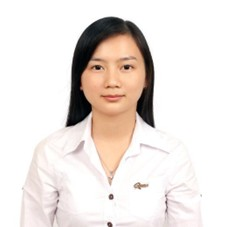
\includegraphics[width=1in,height=1.25in,clip,keepaspectratio]{Authors/ThuNTA.jpg}}]{Thu Nguyen} holds a Master of Science degree in Computer Science from the University of Information Technology, Vietnam National University, Ho Chi Minh City (VNU-HCM). She currently serves as a lecturer in the Faculty of Information Science and Engineering at the University of Information Technology. Her primary research interests encompass Data Science, Artificial Intelligence, and Machine Learning. She has actively contributed to various research projects and has authored publications in reputable international conferences and journals, reflecting her dedication to advancing knowledge in these domains. She can be contacted via email at thunta@uit.edu.vn or n240204@grad.uit.edu.vn.
\end{IEEEbiography}

\begin{IEEEbiography}
[{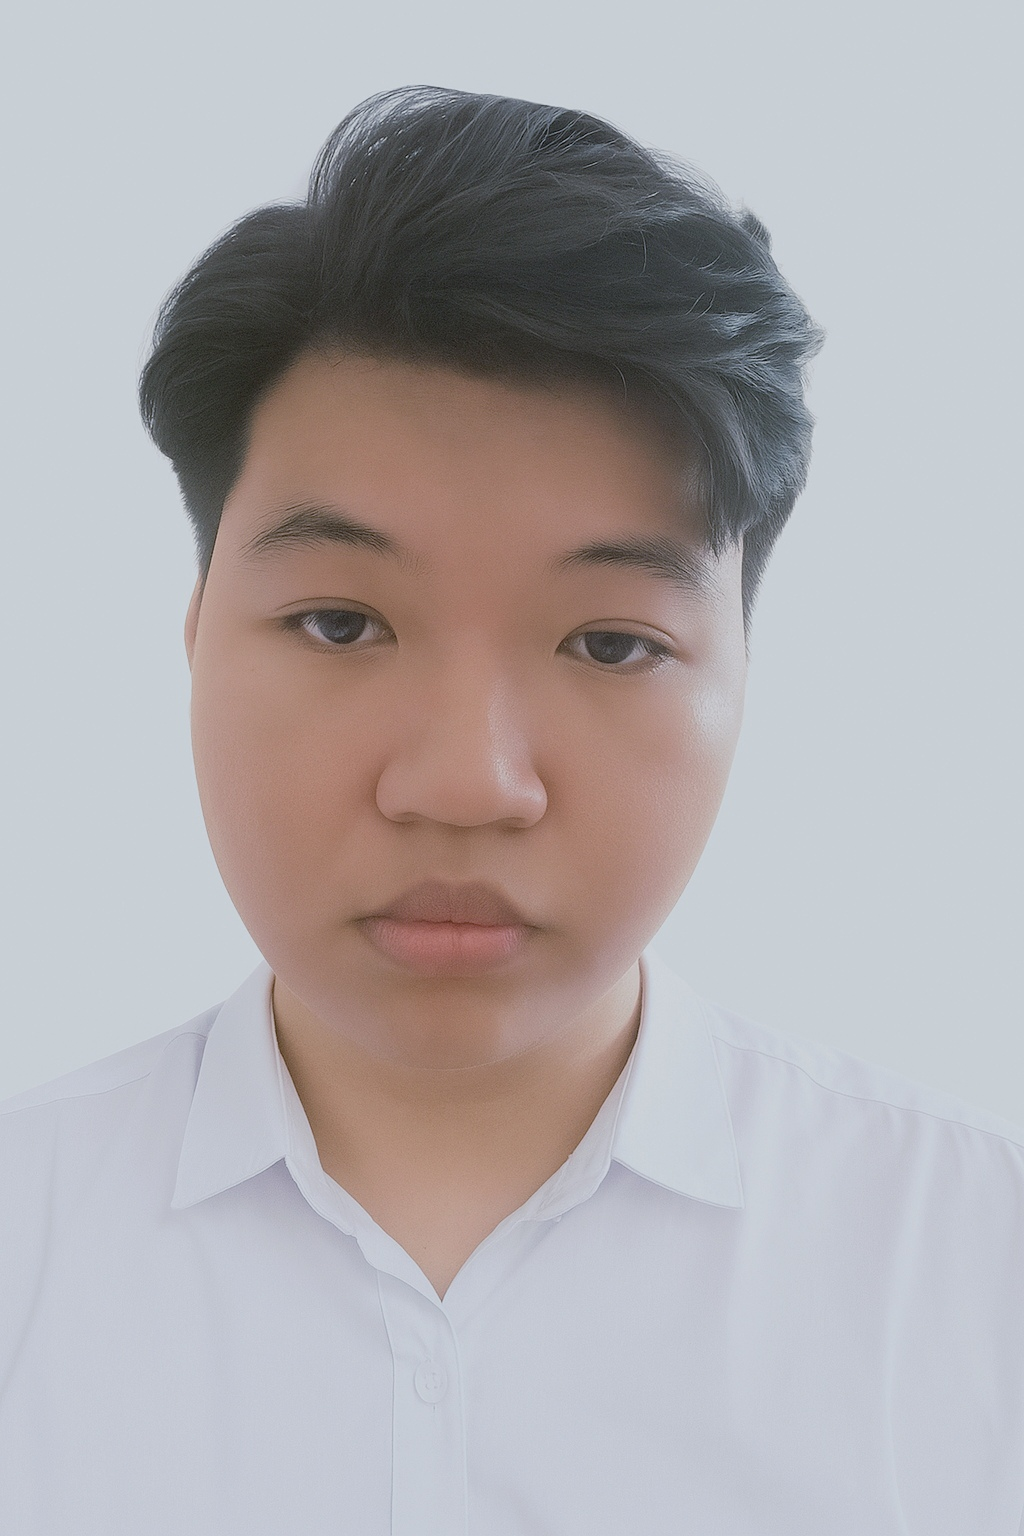
\includegraphics[width=1in,height=1.25in,clip,keepaspectratio]{Authors/DatDT.jpg}}]{Dat Do} is a student majoring in Information Technology at the University of Information Technology, Vietnam National University, Ho Chi Minh City. With a passion for technology, he is particularly interested in the field of machine learning and its practical applications. He continuously strives to learn and research to develop effective technological solutions, contributing to solving real-world problems and advancing progress in this field. You can reach him at 21520694@gm.uit.edu.vn
\end{IEEEbiography}

\begin{IEEEbiography}
[{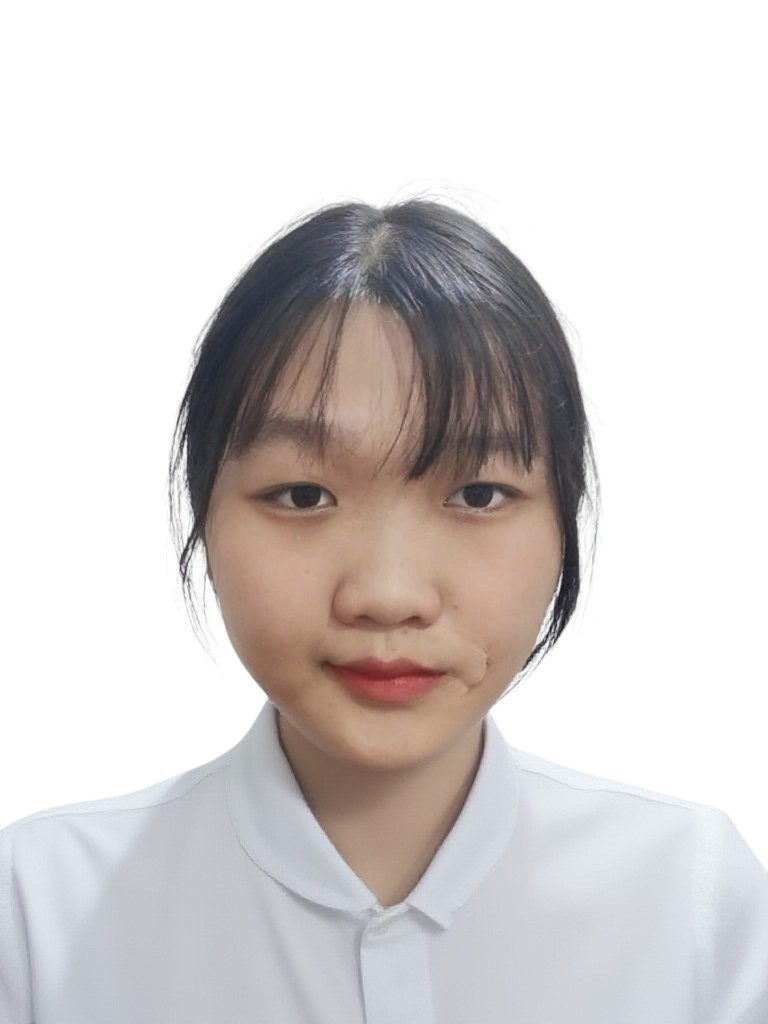
\includegraphics[width=1in,height=1.25in,clip,keepaspectratio]{Authors/HuongVT.jpg}}]{Huong Vi} is currently a student in the Faculty of Information Science and Technology at the University of Information Technology, Vietnam National University, Ho Chi Minh City (VNU-HCM). She is passionate about exploring innovative solutions in information technology and aspires to contribute to the tech industry. You can reach her at 21522132@gm.uit.edu.vn
\end{IEEEbiography}

\begin{IEEEbiography}[{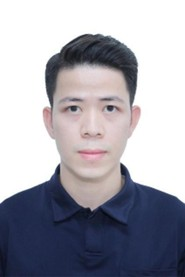
\includegraphics[width=1in,height=1.25in,clip,keepaspectratio]{Authors/KhoaVT.jpg}}]{Khoa Tan VO}, a Master of Science in Information Technology from the University of Information Technology, Vietnam National University, Ho Chi Minh City (VNU-HCM), is a lecturer of the Faculty of Information Science and Engineering at VNU-HCM. Specializing in Software Engineering and Blockchain Technology, he actively contributes to various research projects and has a robust portfolio of publications in prestigious international conferences and journals. His dedication to advancing technology and education underscores his commitment to excellence in his field. You can reach him at khoavt@uit.edu.vn or n240203@grad.uit.edu.vn.
\end{IEEEbiography}

\begin{IEEEbiography}[{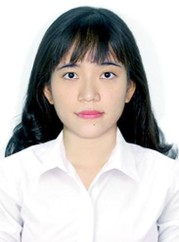
\includegraphics[width=1in,height=1.25in,clip,keepaspectratio]{Authors/ThuyTT.jpg}}]{Thu-Thuy Ta} holds a Master of Science in Computer Science from the University of Information Technology, Vietnam National University, Ho Chi Minh City (VNU-HCM). She is a lecturer of the Faculty of Information Science and Engineering at VNU-HCM. Her research focuses on Data Science and Machine Learning, areas in which she has contributed to several projects and published papers in international conferences and journals. Her work reflects a commitment to advancing the fields of data science and machine learning. You can reach her at thuyta@uit.edu.vn.
\end{IEEEbiography}

\begin{IEEEbiography}[{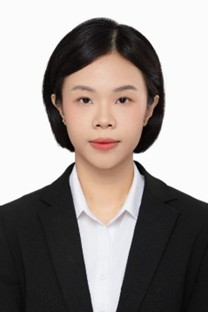
\includegraphics[width=1in,height=1.25in,clip,keepaspectratio]{Authors/ThyNTM.jpg}}]{Mong-Thy Nguyen Thi} holds a Master of Arts in Teaching English as a Second Language (TESL) from Benedictine University, USA. She is an educator at the Center for Foreign Languages, University of Information Technology, Vietnam National University, Ho Chi Minh City (VNU-HCM). Her research focuses on English Language Teaching (ELT) Methodology. Passionate about improving language education, she contributes significantly to advancing ELT practices at her institution. You can reach her at thyntm@uit.edu.vn.
\end{IEEEbiography}

\begin{IEEEbiography}[{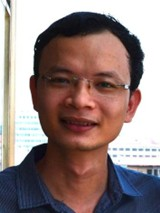
\includegraphics[width=1in,height=1.25in,clip,keepaspectratio]{Authors/PhucNQ.jpg}}]{Phuc Nguyen} received his Master’s degree in Computer Science from the University of Information Technology, a member institution of Vietnam National University, Ho Chi Minh City (VNU-HCM). He is currently serving as a lecturer in the Faculty of Information Systems at the University of Economics and Law, VNU-HCM. His research interests focus on artificial intelligence, business data analytics, and information security. He can be reached via email at phucnq@uel.edu.vn or phucnq.ncs2024@stu.ptit.edu.vn.
\end{IEEEbiography}

\begin{IEEEbiography}[{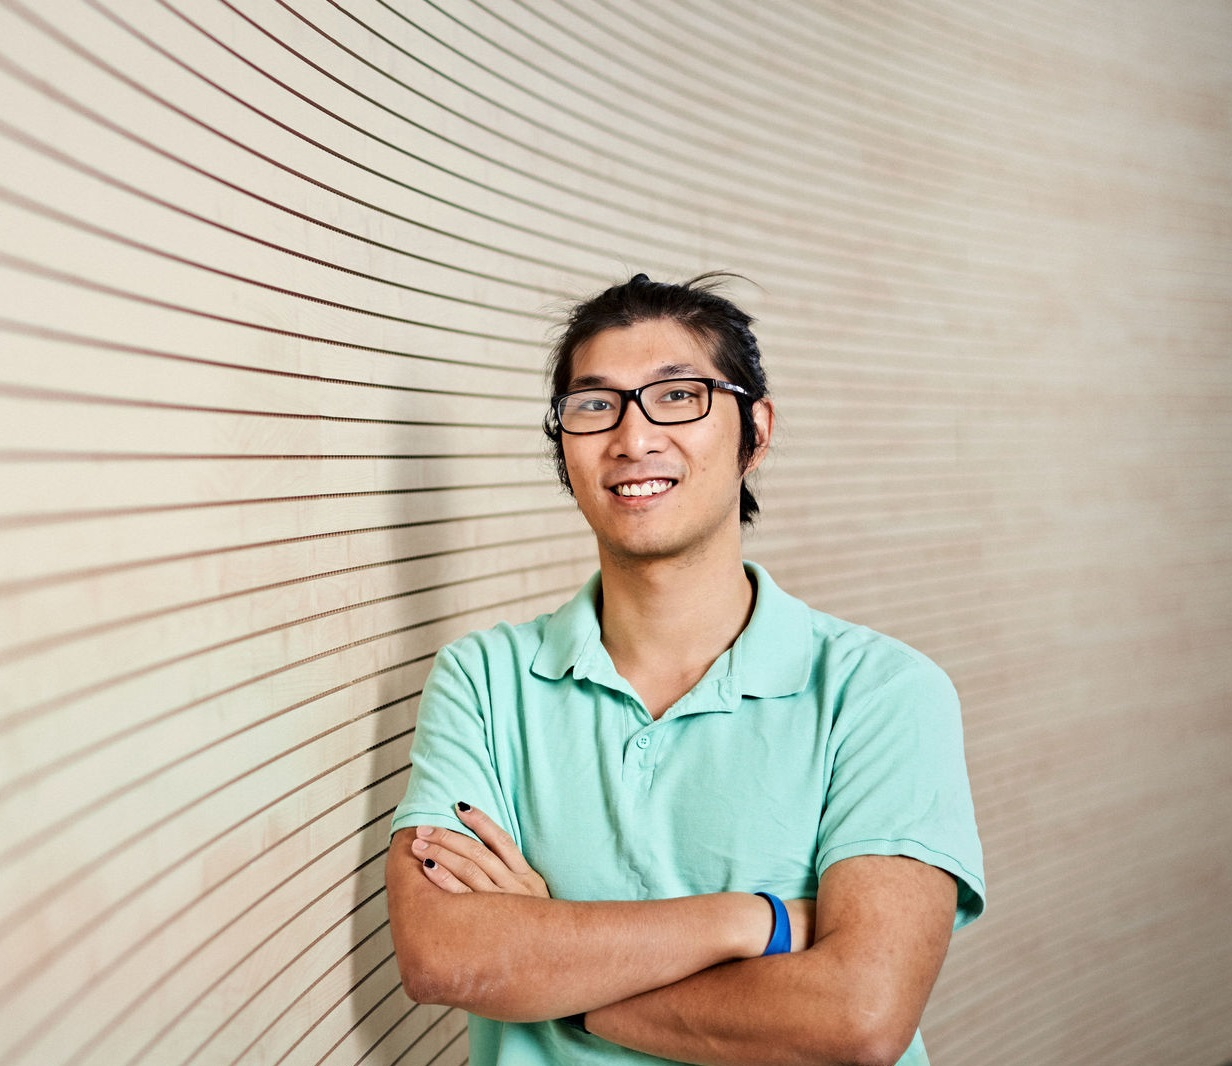
\includegraphics[width=1in,height=1.25in,clip,keepaspectratio]{Authors/TriNH.jpg}}]{Hong-Tri Nguyen} is a postdoctoral researcher at Aalto University. Before Aalto, he received a B.S. degree in computer science from the University of Information Technology -- Vietnam National University, Vietnam, in 2015, and an M.S. degree in computer science from the University of Pisa, Italy, in 2018. Also, he obtained a Ph.D at the University of Oulu in 2023. His research interests include distributed systems, blockchain technology, and information security.
\end{IEEEbiography}

\begin{IEEEbiography}[{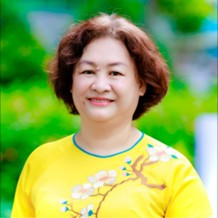
\includegraphics[width=1in,height=1.25in,clip,keepaspectratio]{Authors/AnhNHT.jpg}}]{Tu-Anh Nguyen-Hoang}, Ph.D., is an Associate Professor at the University of Information Technology, Vietnam National University, Ho Chi Minh City (VNU-HCM). She earned her Ph.D. in the Mathematical Foundations of Computer Science and Computational Systems from the University of Science, VNU-HCM. Her research focuses on Data Mining, Soft Computing, and Machine Learning. Dr. Tu-Anh is actively involved in numerous research projects and has a prolific publication record in international conferences and journals. Her work significantly contributes to advancing these specialized fields. You can reach her at anhnht@uit.edu.vn.
\end{IEEEbiography}

\EOD

\end{document}
